\documentclass[12pt]{article}
\usepackage[pdfborder={0 0 0.5 [3 2]}]{hyperref}%
\usepackage[left=1in,right=1in,top=1in,bottom=1in]{geometry}%
\usepackage[shortalphabetic]{amsrefs}%
\usepackage{amsmath}
\usepackage{enumerate}
% \usepackage{enumitem}
\usepackage{amssymb}                
\usepackage{amsmath}                
\usepackage{amsfonts}
\usepackage{amsthm}
\usepackage{bbm}
\usepackage[table,xcdraw]{xcolor}
\usepackage{tikz}
\usepackage{float}
\usepackage{booktabs}
\usepackage{svg}
\usepackage{mathtools}
\usepackage{cool}
\usepackage{url}
\usepackage{graphicx,epsfig}
\usepackage{makecell}
\usepackage{array}

\def\noi{\noindent}
\def\T{{\mathbb T}}
\def\R{{\mathbb R}}
\def\N{{\mathbb N}}
\def\C{{\mathbb C}}
\def\Z{{\mathbb Z}}
\def\P{{\mathbb P}}
\def\E{{\mathbb E}}
\def\Q{\mathbb{Q}}
\def\ind{{\mathbb I}}

\DeclareMathOperator{\spn}{span}
\DeclareMathOperator{\ran}{ran}

\newtheorem{lemma}{Lemma}
\newtheorem{theorem}{Theorem}
\newtheorem{corollary}{Corollary}
\newtheorem{definition}{Definition}
\newtheorem{assumption}{Assumption}
\newtheorem{hypothesis}{Hypothesis}

\newtheorem{notation}{Notation}

\graphicspath{ {discrete/} }

\begin{document}

\section{Introduction}

A lattice dynamical system is an infinite system of ordinary differential equations which are indexed by points in a lattice. For the purposes of this paper, we will only consider dynamical systems on the integer lattice $\Z$, where the differential equation for each point in the lattice is identical and the equations are coupled by a bounded linear operator which involves a finite number of nearby lattice points.

As a specific example, we will look at the discrete nonlinear Schr{\"o}dinger equation (dNLS)
\begin{equation}\label{dNLS}
i\dot{u}_n + \epsilon(u_{n+1} - 2 u_n + u_{n-1}) + |u_n|^2 u_n = 0
\end{equation}
which is (2.12) in \cite{Kevrekidis2009}, where we have taken $\beta = -1$ (focusing) and $\sigma = 1$. The single parameter $\epsilon$ represents the coupling between nodes. We are interested in the existence and stability of standing waves, which are solutions of the form $e^{i \omega t}u_n$. Making this substitution in \eqref{dNLS} and simplifying, we obtain the steady state equation
\begin{equation}\label{dNLSequilib}
\epsilon(u_{n+1} - 2 u_n + u_{n-1}) - \omega u_n + |u_n|^2 u_n = 0
\end{equation}
Taking $u = v + i w$, with $v$ and $w$ real, we obtain the equivalent system of equations
\begin{equation}\label{dNLSequilibreal}
\begin{aligned}
\epsilon (w_{n+1} - 2 w_n + w_{n-1}) + v_n^2 w_n + w_n^3 &= 0 \\
\epsilon (v_{n+1} - 2 v_n + v_{n-1}) + v_n w_n^2 + v_n^3 &= 0
\end{aligned}
\end{equation}
For $\epsilon \neq 0$ we can write \eqref{dNLSequilibreal} as the lattice dynamical system
\begin{equation}\label{DNLSlattice1}
U_{n+1} = F(U_n)
\end{equation}
where $U_n = (v_n, \tilde{v}_n, w_n, \tilde{w}_n)$, $\tilde{v}_n = v_{n-1}$, $\tilde{w}_n = w_{n-1}$, and $F:\R^4 \rightarrow \R^4$ is the smooth function
\begin{equation}\label{FdNLS}
F\begin{pmatrix}
v \\ \tilde{v} \\ w \\ \tilde{w}
\end{pmatrix} =
\begin{pmatrix}
\frac{\omega}{\epsilon} + 2 & -1 & 0 & 0 \\
1 & 0 & 0 & 0 \\
0 & 0 & \frac{\omega}{\epsilon} + 2 & -1 \\
0 & 0 & 1 & 0
\end{pmatrix}
\begin{pmatrix}
v \\ \tilde{v} \\ w \\ \tilde{w}
\end{pmatrix}
- \frac{1}{\epsilon} 
\begin{pmatrix}
v w^2 + v^3 \\ 0 \\ v^2 w + w^3 \\ 0
\end{pmatrix}
\end{equation}

Let $Q_n = (v_n, \tilde{v}_n, w_n, \tilde{w}_n)$ be a solution to \eqref{DNLSlattice1}, so that $u_n = v_n + i w_n$ is a standing wave solution to \eqref{dNLS}. Taking the ansatz $e^{i\omega t} u_n + \eta e^{i\omega t} e^{\lambda t} (a_n + i b_n)$ in \eqref{dNLS}, separating into real and imaginary parts, and writing the resulting equation as a lattice dynamical system, we obtain the eigenvalue problem corresponding to equation \eqref{DNLSlattice1}
\begin{equation}\label{dNLSlatticeEVP}
V_n = DF(Q_n) V_n + \lambda B V_n
\end{equation}
where $V(n) = (a_n, \tilde{a}_n, b_n, \tilde{b}_n)$, $\tilde{a}_n = a_{n-1}$, $\tilde{b}_n = b_{n-1}$, and $B$ is the constant coefficient matrix 
\begin{equation}\label{dNLSB}
B = 
\begin{pmatrix}
0 & 0 & 1 & 0 \\
0 & 0 & 0 & 0 \\
-1 & 0 & 0 & 0 \\
0 & 0 & 0 & 0
\end{pmatrix}
\end{equation}

\section{Main Theorems}

\subsection{Setup}

With dNLS as motivation, we will consider the difference equation
\begin{equation}\label{diffeq}
U(n+1) = F(U(n))
\end{equation}
together with its eigenvalue problem
\begin{equation}\label{latticeEVP}
V(n+1) = DF(U(n)) V(n) + \lambda B V(n)
\end{equation}
where $U(n), V(n) \in \R^d$ for $d \geq 2$, $F: \R^d \rightarrow \R^d$ is a diffeomorphism, $U(n)$ in equation \eqref{latticeEVP} is a solution to \eqref{diffeq}, and $B$ is a $d \times d$ constant matrix. We take the following hypothesis regarding symmetries of $F$.

\begin{hypothesis}\label{symmetryhyp}
There exists a group $G$ for which the group action is a unitary group of symmetries $T(\theta)$ on $\R^d$ such that 
\begin{equation}\label{symmetryrel}
F(T(\theta)U) = T(\theta)F(U)
\end{equation}
for all $\theta \in G$ and all $U \in \R^d$. For the group $G$, we have one of the following:
\begin{enumerate}[(i)]
\item $G$ is a finite group.
\item $G = (\R, +)$.
\end{enumerate}
In addition, for all $\theta$, 
\begin{equation}\label{BTcommute}
B T(\theta) = T(\theta) B
\end{equation}
\end{hypothesis}
If follows from the symmetry relation \eqref{symmetryrel} that $U(n)$ is a solution to \eqref{diffeq} if and only if $T(\theta)U(n)$ is a solution. If we differentiate \eqref{symmetryrel} with respect to $U$, we get the symmetry relation for $DF(U)$
\begin{equation}\label{DFtheta}
D_U F(T(\theta)U) = T(\theta) D_U F(U)T(\theta)^{-1}
\end{equation}
Finally, we note that for Hypothesis \ref{symmetryhyp}(i), the group $G$ can be the trivial group. 

Since we are interested in localized solutions to \eqref{diffeq}, we take the following hypothesis regarding $F$.

\begin{hypothesis}\label{initialhyp}
We assume the following regarding \eqref{diffeq}.
\begin{enumerate}[(i)]
\item 0 is a hyperbolic equilibrium for $F$, thus there exists a radius $r > 1$ such that for all eigenvalues $\nu$ of $DF(0)$, $|\nu| \leq 1/r$ or $|\nu| > r$.
\item $\dim E^s, \dim E^u \geq 1$, where $E^s$ and $E^u$ are the stable and unstable eigenspaces of $DF(0)$.
\item There exists a homoclinic orbit (primary pulse) solution $Q(n)$ to \eqref{diffeq} which connects the equilibrium at 0 to itself.
\end{enumerate}
\end{hypothesis}

Finally, we make the following hypothesis regarding the intersection of the stable manifold $W^s(0)$ and unstable manifold $W^u(0)$. The form of this hypothesis depends on which symmetry hypothesis we choose.

\begin{hypothesis}\label{intersectionhyp}
If Hypothesis \ref{symmetryhyp}(i) holds, the stable and unstable manifolds $W^s(0)$ and $W^u(0)$ intersect transversely.

If Hypothesis \ref{symmetryhyp}(ii) holds, the tangent spaces of the stable and unstable manifolds $W^s(0)$ and $W^u(0)$ have a one-dimensional intersection at $Q(n)$ given by $T'(0) Q(n)$, where $T'(0)$ is the infinitesimal generator of $T(\theta)$.
\end{hypothesis}

\subsection{Existence of Multi-Pulses}

First, we will give criteria for the existence of multi-pulse solutions to \eqref{diffeq}. These solutions resemble multiple, well-separated copies of the primary pulse $Q(n)$. We will characterize such a solution in the following way. Let $m > 1$ be the number of copies of $Q(n)$, and let $N_i$ ($i = 1, \dots, m-1$) be the desired distances (in lattice points) between consecutive copies. Let 
\begin{equation}\label{Nipm}
\begin{aligned}
N_i^+ &= \lfloor \frac{N_i}{2} \rfloor \\
N_i^- &= N_i - N_i^+
\end{aligned}
\end{equation}
and let $N_0^- = N_m^+ = \infty$. Let $N = \min _{i = 1, \dots, m}\{ N_i^\pm \}$. We seek a solution of the form
\begin{align}\label{Upiecewise}
U_i^-(n) &= T(\theta_i) Q(n) + W_i^-(n) && n \in [-N_{i-1}^-, 0] \\
U_i^+(n) &= T(\theta_i) Q(n) + W_i^+(n) && n \in [0, N_i^+]
\end{align}
where $\theta_i = G$ and the pieces are joined together end-to-end as in \cite{Sandstede1998}. The function $W_i^\pm(n)$ is a remainder function which we expect to be small.

In addition to satisfying \eqref{diffeq}, the pieces $U_i^\pm(n)$ must match at the interval endpoints. Thus $U_i^\pm(n)$ must satisfy the system of equations
\begin{equation}\label{Usystem}
\begin{aligned}
(U_i^\pm)(n+1) &= F(U_i^\pm(n))  \\
U_i^+(N_i^+) - U_{i+1}^-(-N_i^-) &= 0 \\
U_i^+(0) - U_i^-(0) &= 0
\end{aligned}
\end{equation}
for $i = 1, \dots, m$. The first equation in \eqref{Usystem} states that the individual pulses are solutions to the difference equation \eqref{diffeq} on the appropriate domains; the second equation glues together the individual pulses at their tails; and the third equation is a matching condition at the centers of the pulses.

Expanding $F$ in a Taylor series about $T(\theta_i) Q(n)$, we get
\begin{align*}
F(U_i^\pm(n)) &= F(T(\theta_i) Q(n) + W_i^\pm(n)) \\
&= F(T(\theta_i) Q(n)) + D_U F(T(\theta_i) Q(n)) W_i^\pm(n) + G(W_i^\pm(n)) \\
&= T(\theta_i)DF(Q(n))T(\theta_i)^{-1} Q(n)) W_i^\pm + G(W_i^\pm(n))
\end{align*}
where $G(W_i^\pm(n)) = \mathcal{O}(|W_i^\pm|^2)$ with $G(0) = 0$ and $DG(0) = 0$, and we used the symmetry relation \eqref{DFtheta} in the last line. Finally, let
\begin{align} \label{didef}
d_i &= T(\theta_{i+1}) Q(-N_i^-) - T(\theta_i) Q(N_i^+)
\end{align}
Substituting these into \eqref{Usystem}, we obtain the following system of equations for the remainder function $W_i^\pm$.
\begin{align}
W_i^\pm(n+1) &= T(\theta)D_U F(Q(n))T(\theta)^{-1} W_i^\pm(n) + G(W_i^\pm(n)) \label{Wsystem1} \\
W_i^+(N_i^+) - W_{i+1}^-(-N_i^-) &= d_i \label{Wsystem2} \\
W_i^+(0) - W_i^-(0) &= 0 \label{Wsystem3}
\end{align}

The variational and adjoint variational equations associated with \eqref{diffeq} come from the linearization of \eqref{diffeq} about the primary pulse solution $Q(n)$, i.e. we take $U(n) = Q(n)$ and $\lambda = 0$ in \eqref{latticeEVP}.
\begin{align}
V(n+1) &= D_U F(Q(n)) V(n) \label{vareq} \\
Z(n+1) &= [D_U F(Q(n))^*]^{-1} Z(n) \label{adjvareq} 
\end{align}
If we take Hypothesis \ref{symmetryhyp}(i), the variational equation does not have a bounded solution, thus we can decompose $\R^d$ as $\R^d = Y^+ \oplus Y^-$, where $Y^+ = T_{Q(0)} W^s(0)$ and $Y^- = T_{Q(0)} W^u(0)$. Since $T(\theta)$ is unitary, we also have the decomposition $\R^d = T(\theta_i) Y^+ \oplus T(\theta_i) Y^-$.

If we instead take Hypothesis \ref{symmetryhyp}(ii), the variational equation \eqref{vareq} has a bounded solution $T'(0) Q(n)$, which can be shown by differentiating $T(\theta) Q(n+1) = F(T(\theta)Q(n))$ with respect to $\theta$ at $\theta = 0$. From Hypothesis \ref{intersectionhyp}, \eqref{vareq} has no other linearly independent bounded solution. Thus we can decompose the tangent spaces to $W^s(0)$ and $W^u(0)$ at $Q(0)$ as
\begin{align*}
T_{Q(0)} W^u(0) &= Y^- \oplus \R T'(0) Q(0) \\
T_{Q(0)} W^s(0) &= Y^+ \oplus \R T'(0) Q(0)
\end{align*}
It also follows from Hypothesis \ref{intersectionhyp} that the adjoint variational equation \eqref{adjvareq} has a unique bounded solution $Z_1(n)$. By Lemma \ref{evolop} below, $Z_1(0) \perp T'(0) Q(0) \oplus Y^- \oplus Y^+$, thus we can decompose $\R^d$ as
\begin{equation}\label{nontdecomp}
\R^d = \R T'(0) Q(0) \oplus Y^+ \oplus Y^- \oplus \R Z_1(0)
\end{equation}
Since $T(\theta)$ is unitary, we also have the decomposition
\begin{equation}\label{nontdecompT}
\R^d = \R T(\theta_i) T'(0) Q(0) \oplus T(\theta_i) Y^+ \oplus T(\theta_i) Y^- \oplus \R T(\theta_i) Z_1(0)
\end{equation}
Finally, since perturbations in the direction of $T(\theta_i) T'(0) Q(0)$ are handled by the symmetry parameter $\theta_i$, we may without loss of generality choose $W_i^\pm$ so that 
\begin{equation}\label{W0loc}
W_i^\pm(0) \in T(\theta_i) Y^+ \oplus T(\theta_i) Y^- \oplus \R T(\theta_i) Z_1(0)
\end{equation}

We can now state the following theorems regarding existence of multi-pulse solutions to \eqref{diffeq}. Proofs of the theorems will follow in a later section. First, if Hypothesis \ref{symmetryhyp}(i) holds, we have a unique $m-$pulse solution to \eqref{diffeq}.

\begin{theorem}\label{transversemulti}
Assume Hypotheses \ref{symmetryhyp}(i), \ref{initialhyp}, and \ref{intersectionhyp}, and let $Q(n)$ be the primary pulse solution to \eqref{diffeq}. Then, for sufficiently large $N$, there exists a unique $m-$pulse solution $Q_m(n)$ to \eqref{diffeq} which can be written piecewise in the form \eqref{Upiecewise}. For the remainder terms $W_i^\pm(n)$ we have the following estimates
\begin{equation}\label{Westimates}
\begin{aligned}
||W_i^\pm|| &\leq C r^{-N} \\
W_i^+(N_i^+) &= T(\theta_{i+1}) Q(-N_i^-) + \mathcal{O}(r^{-2N}) \\
W_{i+1}^-(-N_i^-) &= T(\theta_i) Q(N_i^+) + \mathcal{O}(r^{-2N})
\end{aligned}
\end{equation}
\end{theorem}

If \ref{symmetryhyp}(ii) holds, we will not in general have a solution to \eqref{diffeq}, since Lin's method gives us a solution with $m$ jumps in the direction of $Z_1(0)$. Instead, we give a criterion for such a solution to exist, which amounts to these $m$ jumps being 0.

\begin{theorem}\label{ntmulti}
Assume Hypotheses \ref{symmetryhyp}(ii), \ref{initialhyp}, and \ref{intersectionhyp}, and let $Q(n)$ be the primary pulse solution to \eqref{diffeq}. Then, for sufficiently large $N$, there exists a unique $m-$pulse solution $Q_m(n)$ to \eqref{diffeq} if and only if $m$ jump conditions 
\begin{align}\label{jumpcondexist}
\xi_i &= \langle T(\theta_i) Z_1(N_i^+), T(\theta_{i+1}) Q(-N_i^-) \rangle
- \langle T(\theta_i) Z_1(-N_{i-1}^-), T(\theta_{i-1}) Q(N_{i-1}^+) \rangle + R_i = 0 && i = 1, \dots, m
\end{align}
are satisfied, where $\langle T(\theta_m) Z_1(N_m^+), T(\theta_{m+1}) Q(-N_m^-) \rangle = 0$, $\langle T(\theta_1) Z_1(-N_0^-), T(\theta_0) Q(N_0^+) \rangle = 0$, and the remainder terms have uniform bound
\[
|R_i| \leq C r^{-3N}
\]
$Q_m(n)$ can be written piecewise in the form \eqref{Upiecewise}, and the estimates \eqref{Westimates} on $W_i^\pm$ from Theorem \ref{transversemulti} hold in this case.
\end{theorem}

\subsection{Stability Problem}

We will now look at the spectral stability of multi-pulse solutions to \eqref{diffeq}. In this section, we will always assume Hypotheses \ref{symmetryhyp}(ii). Suppose we have successfully used Theorem \ref{ntmulti} to construct an $m-$pulse solution $Q_m(n)$ to \eqref{diffeq}, which we can write piecewise as
\begin{align}\label{qmpiecewise}
Q_m(n) =
\begin{cases}
T(\theta_i) Q(n) + \tilde{Q}_i^-(n) & n = [-N_{i-1}^-, 0] \\
T(\theta_i) Q(n) + \tilde{Q}_i^+(n) & n = [0, N_i^+] \\
\end{cases}
\end{align}
For the eigenvalue problem, we take $U(n) = Q_m(n)$ in equation \eqref{latticeEVP} to get
\begin{equation}\label{multiEVP}
V(n+1) = DF(Q_m(n)) V(n) + \lambda B V(n)
\end{equation}
Since $Q_m(n)$ decays exponentially to 0 and $F$ is smooth, $DF(Q_m(n))$ is exponentially asymptotic to the constant coefficient matrix $DF(0)$, which is hyperbolic by Hypothesis \ref{initialhyp}. 

We will also assume one of the following Melnikov sum conditions holds.
\begin{hypothesis}\label{melnikovhyp}
One of the following Melnikov conditions holds.
\begin{enumerate}[(i)]
\item
\begin{equation}\label{M1cond}
M_1 = \sum_{n=-\infty}^\infty \langle Z_1(n+1), B T'(0)Q(n) \rangle \neq 0
\end{equation}
\item $M_1 = 0$, and there exists a function $S_1(n)$ such that
\begin{equation}\label{S1def}
S_1(n+1) = DF(Q(n)) S_1(n) + B T'(0)Q(n)
\end{equation}
and 
\begin{equation}\label{M2cond}
M_2 = \sum_{n=-\infty}^\infty \langle Z_1(n+1), B S_1(n) \rangle \neq 0 
\end{equation}
Furthermore, $S_1(n)$ is exponentially localized with decay rate
\begin{equation}\label{S1decay}
|S_1(n)| \leq C r^{-|n|}
\end{equation}
\end{enumerate}
\end{hypothesis}
For Hamiltonian systems, the existence of $S_1(n)$ in Hypothesis \ref{melnikovhyp}(ii) is a consequence of the following lemma.

\begin{lemma}
The following conditions...
\begin{enumerate}
\item The stable manifold $W^s(0)$ and the unstable manifold $W^u(0)$ intersect transversely in $H^{-1}(0)$ at $Q(0)$.
\end{enumerate}
\end{lemma}

We can now state the stability theorem, in which we locate the eigenvalues of \eqref{latticeEVP} resulting from interactions between neighboring pulses.

\begin{theorem}\label{stabilitytheorem}
Assume Hypotheses \ref{symmetryhyp}(ii), \ref{initialhyp}, \ref{intersectionhyp}, and let $Q_m(n)$ an $m-$pulse solution to \eqref{diffeq} constructed according to Theorem \ref{ntmulti}. Then there exists a bounded, nonzero solution $V(n)$ of the eigenvalue problem \eqref{multiEVP} for $|\lambda| < \delta$ if and only if $\det E(\lambda) = 0$, where
\begin{equation}\label{Elambda}
E(\lambda) = \begin{cases}
\det(A - M_1 \lambda I + R(\lambda))
& \text{Hypothesis \ref{melnikovhyp}(i) holds} \\
\det(A - M_2 \lambda^2 I + R(\lambda))
& \text{Hypothesis \ref{melnikovhyp}(ii) holds}
\end{cases}
\end{equation}
$M_1$ and $M_2$ are defined in Hypothesis \eqref{melnikovhyp}. $A$ is the tridiagonal $m \times m$ matrix
\begin{align}\label{matrixA}
A &= \begin{pmatrix}
-a_1 & a_1 & & &  \\
-\tilde{a}_1 & \tilde{a}_1 - a_2 & a_2 \\
& -\tilde{a}_2 & \tilde{a}_2 - a_3 & a_3 \\
& \ddots & & \ddots \\
& & & -\tilde{a}_{m-1} & \tilde{a}_{m-1}  \\
\end{pmatrix}
\end{align}
where
\begin{align*}
a_i &= \langle T(\theta_i) Z_1(N_i^+), T(\theta_{i+1}) T'(0)Q(-N_i^-) \rangle \\
\tilde{a}_i &= \langle T(\theta_{i+1}) Z_1(-N_i^-), T(\theta_i) T'(0)Q(N_i^+) \rangle
\end{align*}
and the remainder term has uniform bound
\begin{align}\label{Rbound2}
|R(\lambda)| \leq C\left( (r^N + |\lambda|)^3 \right)
\end{align}
\end{theorem}

\section{Discrete NLS}

\subsection{Background}

In this section, we will apply the results the previous section to the discrete NLS equation \eqref{dNLS}. Before we do that, we will give a brief overview of the equation and what is already known. More details can be found in \cite{Kevrekidis2009}. 

Equation \eqref{dNLS} is Hamiltonian, with energy given by (2.17) in \cite{Kevrekidis2009}. Alternatively, taking $u = v + i w$, with $v$ and $w$ real, we can write \eqref{dNLS} in Hamiltonian form as
\begin{equation}\label{dNLSrealHam}
\frac{d}{dt}\begin{pmatrix}v_n \\ w_n\end{pmatrix}
+ J \nabla H(u_n, v_n) = 0
\end{equation}
where $J$ is the standard skew-symmetric symplectic matrix
\[
J = \begin{pmatrix}0 & 1 \\ -1 & 0\end{pmatrix}
\]
and the Hamiltonian $H$ is
\begin{equation}\label{dNLSrealH}
H(u_n, v_n) = -\sum_{n = -\infty}^\infty 
\left( \frac{1}{2}\left(v_n - v_{n-1}\right)^2 + \frac{1}{2}\left(w_n - w_{n-1}\right)^2 - \frac{1}{4}\left( v_n^2 + w_n^2 \right)^2 \right)
\end{equation}

At the anti-continuum limit, when $\epsilon = 0$, equation \eqref{dNLSequilib} reduces to a system of decoupled algebraic equations. Any function $u(n)$ with $u(n) \in \{ 0, \pm \sqrt{\omega}\}$ is a solution. For $\epsilon > 0$, dNLS possesses two real-valued, symmetric, single pulse solutions (up to rotation): on-site solutions, which are centered on a single lattice point; and off-site solutions, which are centered between two adjacent lattice points \cite{Kevrekidis2009}. The on-site solution has a single eigenvalue at 0 from the rotational symmetry. The off-site solution has an additional pair of real eigenvalues; since the off-site solution is spectrally unstable, we will only consider the on-site solution from here on. 

Let $q(n)$ be the on-site solution to \eqref{dNLSequilib}, which exists for all $\epsilon > 0$ (REFERENCE). For sufficiently small $\epsilon$, $m$-pulse solutions exist for any pulse distances $N_i^\pm$ and any phase differences $\Delta \theta_i \in \{0, \pi\}$ \cite[Proposition 2.1]{Pelinovsky2005}. For sufficiently small $\epsilon$, this $m-$pulse is spectrally unstable unless all of the phase differences $\Delta \theta_i$ are $\pi$; in that case there are $m-1$ pairs of purely imaginary eigenvalues with negative Krein signature \cite[Theorem 3.6]{Pelinovsky2005}. For any $\epsilon$ for which the $m-$pulse exists, if one or more phase differences $\Delta \theta_i$ is 0, it follows from Sturm-Liouville theory that there is at least one positive, real eigenvalue \cite{Kapitula2001a}.

\subsection{Real-valued multi-pulses}

We will now show existence of multi-pulse solutions. First, we will look for real-valued solutions to \eqref{dNLSequilib}. In this case, the stationary equation reduces to
\begin{equation*}
\epsilon(u_{n+1} - 2 u_n + u_{n-1}) - \omega u_n + u_n^3 = 0
\end{equation*}
For $\epsilon \neq 0$, this is equivalent to the first order difference equation $U_{n+1} = F(U_n)$, where $U_n = (u_n, \tilde{u}_n) \in \R^2$, $\tilde{u}_n = u_{n-1}$, and 
\begin{equation}\label{dnlsdiffR2}
F
\begin{pmatrix}
u \\ \tilde{u}
\end{pmatrix} =
\begin{pmatrix}
\frac{\omega}{\epsilon} + 2 & -1 \\
1 & 0
\end{pmatrix}
\begin{pmatrix}
u \\ \tilde{u}
\end{pmatrix}
- \frac{1}{\epsilon} 
\begin{pmatrix}
u^3 \\ 0
\end{pmatrix}
\end{equation}
The symmetry group $G = \{ 1, -1\}$ acts on $\R^2$ via $T(\theta) = \theta I$, thus Hypothesis \ref{symmetryhyp}(i) is satisfied. For $\epsilon, \omega > 0$, $DF(0)$ has a pair of real eigenvalues $\{r, 1/r \}$, where $r$ depends on both $\epsilon$ and $\omega$, and is given by
\begin{align}\label{defr}
r = 1 + \frac{\omega}{2 \epsilon} \left( 1 + \sqrt{1 + \frac{4 \epsilon}{\omega}} \right) > 1
\end{align}
As $\epsilon \rightarrow \infty$, $r \rightarrow 1$, thus the spectral gap decreases with increasing $\epsilon$. As $\epsilon \rightarrow 0$, $r \rightarrow \infty$.

It follows that 0 is a hyperbolic equilibrium point with 1-dimensional stable and unstable manifolds. Let $q_n$ be the on-site, real-valued solution to \eqref{dNLSequilib}. Then $Q_n = (q_n, \tilde{q}_n)$ is the primary pulse solution to $U_{n+1} = F(U_n)$, where $\tilde{q}_n = q_{n-1}$. Thus Hypothesis \ref{initialhyp} is satisfied. Since the variational equation does not have a bounded solution, the stable and unstable manifolds intersect transversely, thus Hypothesis \ref{intersectionhyp} is satisfied. 

Using Theorem \ref{transversemulti}, for sufficiently large $N$ (which depends on $r$, thus $\omega$ and $\epsilon$) there exist $m-$pulse solutions for any $\theta_i = \pm 1$ and lengths $N_i \geq N$. 

\subsection{No other multi-pulses}

We will now show that (up to rotation), there are no other multi-pulse soliton solutions to dNLS, i.e. there are no multi-pulse solutions with phase differences other than $0$ and $\pi$. For convenience, we will reuse much of the notation from the previous section. In this case, $u$ can be complex, so for $\epsilon \neq 0$, we are looking for solutions to the difference equation 
\begin{equation}\label{dNLSdiff}
U(n+1) = F(U(n))
\end{equation}
where $U(n) \in \R^4$ and $F$ is defined in equation \eqref{FdNLS}. The symmetry group $G = (\R, \cdot)$ acts on $\R^4$ via $T(\theta)$, where
\begin{align}\label{TdNLS}
T(\theta) =
\begin{pmatrix}
\cos\theta & 0 &-\sin\theta & 0 \\
0 & \cos\theta & 0 &-\sin\theta \\
\sin\theta & 0 & \cos\theta & 0 \\
0 & \sin\theta & 0 & \cos\theta 
\end{pmatrix}
\end{align}
which has infinitesimal generator
\begin{align}\label{dnlsSgen}
T'(0) =
\begin{pmatrix}
0 & 0 &-1 & 0 \\
0 & 0 & 0 &-1 \\
1 & 0 & 0 & 0 \\
0 & 1 & 0 & 0 
\end{pmatrix}
\end{align}

For $\epsilon, \omega > 0$, $DF(0)$ has eigenvalues $\{r, 1/r\}$, each of which has multiplicity 2; the constant $r$ is defined in equation \eqref{defr} in the previous section. Thus $DF(0)$ is hyperbolic and has 2-dimensional stable and unstable manifolds. Let $q(n)$ be the real-valued, on-site, primary pulse solution to \eqref{dNLSequilib}. Then the primary pulse solution to $U_{n+1} = F(U_n)$ is given by $Q(n) = (q(n), \tilde{q}(n), 0, 0)$. Thus Hypothesis \ref{initialhyp} is satisfied.

The variational and adjoint variational equations associated with \eqref{dNLSdiff} are
\begin{align}
V(n+1) &= D_U F(Q(n)) V(n) \label{vareqdNLS} \\
Z(n+1) &= [D_U F(Q(n))^*]^{-1} Z(n) \label{adjvareqdNLS}
\end{align}
We can verify that $T'(0) Q(n) = (0, 0, q(n), \tilde{q}(n))$ is a solution to \eqref{vareqdNLS}, as expected. From [CITATION OR HYPOTHESIS], there are no other linearly independent, bounded solutions to \eqref{vareqdNLS}, thus Hypothesis \ref{intersectionhyp} is satisfied. It follows the the adjoint variational equation \eqref{adjvareqdNLS} has a unique bounded solution $Z_1(n)$, and we can verify directly that
\begin{equation}\label{defZ1}
Z_1(n) = (0, 0, -\tilde{q}(n), q(n))
\end{equation}

Using Theorem \ref{ntmulti}, for sufficiently large $N$ (which depends on $r$, thus $\omega$ and $\epsilon$) there exist $m-$pulse solutions with lengths $N_i^\pm$ and phase parameters $\theta_i$ if any only if the jump conditions \eqref{jumpcondexist} are satisfied. Using \eqref{TdNLS} and the fact that $T(\theta)$ is unitary, we can rewrite the jump conditions in terms of the $(m - 1)$ phase differences $\Delta \theta_i = \theta_{i+1} - \theta_i$ to get
\begin{align}\label{jumpDNLS}
\xi_i = \langle T(-\Delta \theta_i) Z_1(N_i^+), Q(-N_i^-) \rangle
- \langle T(\Delta \theta_{i-1}) Z_1(-N_{i-1}^-), Q(N_{i-1}^+) \rangle + R_i
\end{align}
where $\Delta \theta_0 = 0$ and $\Delta \theta_m = 0$. The inner product terms in \eqref{jumpDNLS} are
\begin{equation}\label{jumpIPs}
\begin{aligned}
\langle T(-\Delta\theta_i) Z_1(N_i^+), Q(-N_i^-) \rangle 
&= -b_i \sin(\Delta\theta_i) \\
\langle T(\Delta\theta_{i-1}) Z_1(-N_{i-1}^-), Q(N_{i-1}^+) \rangle &= -b_{i-1} \sin(\Delta\theta_{i-1})
\end{aligned}
\end{equation}
where 
\begin{align*}
b_i &= q(N_i^+ - 1)q(N_i^-) - q(N_i^+)q(N_i^- + 1) \\
\end{align*}
Since the single pulse $q(n)$ is an even function, we can write $b_i$ as
\begin{equation}\label{bieq}
b_i = \begin{cases}
q(N_i^+)\left( q(N_i^+ + 1) - q(N_i^+ - 1) \right) & N_i \text{ even} \\
q(N_i^+)q(N_i^+ + 2) - q(N_i^+ - 1)q(N_i^+ + 1) & N_i \text{ odd}
\end{cases}
\end{equation}
Since $q(n)$ is strictly decreasing as $n$ moves away from 0 [CITATION, THIS IS TRUE FOR SUFFICIENTLY LARGE $N$ SINCE $r$ IS REAL, AND I BELIEVE IT IS ALWAYS TRUE], $b_i < 0$ for all $i$. 

Letting $s_i = \sin{\Delta\theta_i}$ and substituting equations \eqref{jumpIPs} into \eqref{jumpDNLS}, the jump conditions become
\begin{equation}\label{jumpDNLS2}
\begin{aligned}
\xi_1 &= -b_1 s_1 + R_1 \\
\xi_i &= b_{i-1} s_{i-1} - b_i s_i + R_i
&& i = 2, \dots, m-1 \\
\xi_m &= b_{m-1} s_{m-1} + R_m
\end{aligned}
\end{equation}
Since $b_i = \mathcal{O}(r^{-2N})$ and $R_i = \mathcal{O}(r^{-3N})$, the jump conditions can only be satisfied if $s_i = \mathcal{O}(r^{-N})$. Thus we only have to consider that case from now on. 
 
There exists a conserved quantity $E: \R^4 \rightarrow \R$ such that $E(0) = 0$ and $E(U_{n+1}) = E(U_n)$ for all solutions $U_n$ to \eqref{dNLSdiff} [EITHER FIND CITATION OR ACTUALLY FIND IT]. Thus, as in \cite{SandstedeStrut}, we can eliminate the final equation in \eqref{jumpDNLS2}. We can write the $(m-1)$ remaining jump conditions in matrix form as $H s + R = 0$, where $s = (s_1, \dots, s_{m-1})$ and $B$ is the $(m-1)\times(m-1)$ matrix
\[
H = \begin{pmatrix}
-b_1 \\
b_1 & -b_2 \\
& b_2 & -b_3 \\
&& \ddots & \ddots \\
&&& b_{m-2} & -b_{m-1} \\
\end{pmatrix}
\]
Since $H$ is lower triangular and all the $b_i$ are nonzero, $B$ is invertible, thus $s = B^{-1}R$ is the unique value of $s$ for which all the jump conditions are satisfied. In the previous section, we showed that for sufficiently large $N$, real-valued multi-pulses exist with phase differences which are either 0 or $\pi$; for all of those cases, $s = 0$. Since we found a unique solution $s$, and $s = 0$ is a solution, $s = 0$ must be the unique solution to the jump conditions. We conclude that for sufficiently large $N$, the jump conditions can only be satisfied if all of the phase differences $\Delta \theta_i$ are either 0 or $\pi$. No other phase differences are possible.

\subsection{Eigenvalue problem}

In this section, we locate the eigenvalues for the linearization of \eqref{dNLS} about the multi-pulse $Q_m(n)$, i.e. we solve equation \eqref{multiEVP} with $B$ defined in \eqref{dNLSB}. We can show directly that $B T(\theta) = T(\theta) B$. We showed in the previous section that $T'(0)Q(n)$ is the unique bounded solution to the variational equation \eqref{vareqdNLS}, and that $Z_1(n)$ is the unique bounded solution to the adjoint variational equation \eqref{adjvareqdNLS}. For the first Melnikov sum, we have
\[
M_1 = \sum_{n=-\infty}^\infty \langle Z_1(n+1), B T'(0)Q(n) \rangle = 0
\]
Let 
\begin{align}\label{dNLSdefS1}
S_1 &= (-\partial_\omega q_n, -\partial_\omega \tilde{q}_n, 0, 0)
\end{align}
It is straightforward to verify that
\begin{align*}
S_1(n+1) &= DF(Q(n)) S_1(n) + B T'(0) Q(n)
\end{align*}
The higher order Melnikov sum is
\[
M_2 = \sum_{n=-\infty}^\infty \langle Z_1(n+1), B S_1(n) \rangle =
\sum_{n=-\infty}^\infty q(n) q_\omega(n)
\]
Numerical analysis suggests that $M_2 > 0$, so we will assume that is the case. Thus Hypothesis \ref{melnikovhyp}(ii) is satisfied.

For $N$ sufficiently large, we can find the eigenvalues of \eqref{multiEVP} using Theorem \ref{stabilitytheorem}. The matrix $A$ is
\begin{align}\label{AdNLS}
A &= \begin{pmatrix}
-\cos(\Delta\theta_1) b_1 & \cos(\Delta\theta_1) b_1 & & &  \\
\cos(\Delta\theta_1) b_1 & -\cos(\Delta\theta_1) b_1 - \cos(\Delta\theta_2) b_2 & \cos(\Delta\theta_2) b_2 \\
& \ddots & \ddots \\
& &  \cos(\Delta\theta_{m-1}) b_{m-1} & -\cos(\Delta\theta_{m-1}) b_{m-1}  \\
\end{pmatrix}
\end{align}
where the $b_i < 0$ and are defined in \eqref{bieq}. To solve $E(\lambda) = 0$, we need to find the eigenvalues of $A$. Since $A$ is symmetric tridiagonal, its eigenvalues are real. Furthermore, $A$ has an eigenvalue at 0 with corresponding eigenvector $(1, 1, \dots, 1)^T$. Using \cite[Lemma 5.4]{Sandstede1998}, the signs of the remaining $m-1$ eigenvalues of $A$ are determined by the phase differences $\Delta\theta_i$.  
\begin{enumerate}
	\item $A$ has $k_\pi$ negative real eigenvalues (counting multiplicity), where $k_\pi$ is the number of $\Delta\theta_i$ which are $\pi$. 
	\item $A$ has $k_0$ positive real eigenvalues (counting multiplicity), where $k$ is the number of $\Delta\theta_i$ which are $0$. 
\end{enumerate}
To show that the eigenvalues of $A$ are distinct, we note that $\mu$ is an eigenvalue of $A$ if and only if $(A - \mu I)v = 0$ has a nontrivial solution. Let $p_i = \cos(\Delta\theta_i) b_i$. Then the equation $(A - \mu I)v = 0$ can be written as the Sturm-Liouville difference equation with Dirichlet boundary conditions
\begin{equation}\label{SLdiff2}
\begin{aligned}
\nabla( p_j \Delta d_j ) &= \mu d_j && j = 1, \dots, m \\
d_0 &= 0 \\
d_{m+1} &= 0
\end{aligned}
\end{equation}
where $\Delta$ is the forward difference operator $\Delta f(j) = f(j+1) - f(j)$ and $\nabla$ is the backward difference operator $\nabla f(j) = f(j) - f(j-1)$. It follows from \cite[Corollary 2.2.7]{Jirari1995} that the eigenvalues of \eqref{SLdiff2}, thus the eigenvalues of $A$, are real and distinct. Let $\{0, \mu_1, \dots, \mu_{m-1}\}$ be the distinct eigenvalues of $A$.

To find the eigenvalues of \eqref{multiEVP}, we will solve equation \eqref{Elambda}. We will always have an eigenvalue at 0 with algebraic multiplicity 2 and geometric multiplicity 1. We can verify directly that $T'(0) Q_m(n)$ is the eigenfunction and $S_m(n) = \partial_\omega Q_m(n)$ is the generalized eigenfunction. The remaining eigenvalues result from interaction between the pulses. To find these, we rescale equation \eqref{Elambda} in the following way. Let
\begin{align*}
A = r^{-2N} \tilde{A} \\
\lambda = r^{-N} \tilde{\lambda} \\
R(\lambda) = r^{-3N} \tilde{R}(\lambda)
\end{align*}
The eigenvalues of $\tilde{A}$ are $\{0, \tilde{\mu}_1, \dots, \tilde{\mu}_{m-1}\}$, which are distinct, and $\mu_j = r^{-2N} \tilde{\mu_j}$. Dividing by $r^{-2N}$, solving \eqref{Elambda} is equivalent to solving
\[
\det(\tilde{A} - M_2 \tilde{\lambda}^2 I + r^{-N} \tilde{R}(\lambda)) = 0
\]

Let $\epsilon = r^{-N}$, and let
\begin{equation}\label{deftildeE}
\tilde{E}(\tilde{\lambda}; \epsilon) = \det(\tilde{A} - M_2 \tilde{\lambda}^2 I + \epsilon \tilde{R}(\lambda))
\end{equation}
For $j = 1, \dots, m-1$, $\tilde{E}(\pm \sqrt{\tilde{\mu}_j / M_2 }; 0) = 0$. Since the eigenvalues of $\tilde{A}$ are distinct, 
\[
\frac{\partial}{\partial \tilde{\lambda}} \tilde{E}(\tilde{\lambda}; 0)\Big|_{\tilde{\lambda} = \pm \sqrt{\tilde{\mu}_j / M_2 }} \neq 0
\]
Using the IFT, we can solve for $\tilde{\lambda}$ as a function of $\epsilon$ near $(\tilde{\lambda}, \epsilon) = (\pm \sqrt{\tilde{\mu}_j / M_2 }; 0)$. Thus for sufficiently small $\epsilon$, we can find smooth functions $\tilde{\lambda}_j^\pm(\epsilon)$ such that $\tilde{\lambda}_j^\pm(0) = \pm \sqrt{\tilde{\mu}_j / M_2 }$ and $E(\tilde{\lambda}_j^\pm(\epsilon); \epsilon) = 0$. 

Expanding $\tilde{\lambda}(\epsilon)$ in a Taylor series about $\epsilon = 0$ and taking $\epsilon = r^{-N}$, we can write $\tilde{\lambda}_j^\pm$ as a function of $N$ to get 
\begin{equation*}
\tilde{\lambda}_j^\pm(N) = \tilde{\lambda}_j^\pm + \mathcal{O}(r^{-N})
\end{equation*}
Undoing the scaling, the interaction eigenvalues are given by
\begin{align*}
\lambda^\pm_j(N) &= \pm \sqrt{\frac{\tilde{\mu}_j}{M_2}} r^{-N} + \mathcal{O}(r^{-2N}) && j = 1, \dots, m-1 
\end{align*}

Since \eqref{dNLS} is Hamiltonian, by Hamiltonian symmetry, eigenvalues must come in quartets $\pm a \pm i b$. Since the $\mu_j$ are distinct and only come in pairs, the eigenvalues $\lambda^\pm(N)$ must be either real or purely imaginary. We conclude that there are $(m - 1)$ pairs of nonzero interaction eigenvalues at $\lambda = \pm \lambda_j(N)$ given by 
\begin{align}\label{inteigsDNLS}
\lambda_j(N) &= \sqrt{\frac{\tilde{\mu}_j}{M_2}}r^{-N} + \mathcal{O}(r^{-2N}) && j = 1, \dots, m-1
\end{align}
These are either real or purely imaginary, and the remainder term cannot move these off of the real or imaginary axis. Since $M_2 > 0$, we conclude that there are
\begin{enumerate}
	\item $k_\pi$ pairs of purely imaginary eigenvalues
	\item $k_0$ pairs of real eigenvalues
\end{enumerate}

Finally, we consider three special cases. The simplest case is the 2-pulse. The matrix $A$ is given by
\begin{align*}
A &= b_1 \begin{pmatrix}
-\cos(\Delta\theta_1) & \cos(\Delta\theta_1) \\
\cos(\Delta\theta_1) & -\cos(\Delta\theta_1) 
\end{pmatrix}
\end{align*}
which has nonzero eigenvalue $-\cos(\Delta\theta_1) b_1$, thus there is a pair of interaction eigenvalues given by
\begin{align*}
\lambda &= \sqrt{\frac{-\cos(\Delta\theta_1) b_1}{M_2}} + \mathcal{O}(r^{-2N})
\end{align*}
Since $b_1 < 0$ and $M_2 > 0$, this pair is real if $\Delta\theta_1 = 0$ and purely imaginary if $\Delta\theta_1 = \pi$.

Next, we consider the 3-pulse with equal distances $N_1 = N_2$, so we have $b_1 = b_2 = b$. There are three distinct combinations of $(\Delta\theta_1, \Delta\theta_2)$ to consider. The matrix $A$ is given by
\begin{align*}
A &= b \begin{pmatrix}
-\cos(\Delta\theta_1) & \cos(\Delta\theta_1) & 0  \\
\cos(\Delta\theta_1) & -\cos(\Delta\theta_1) - \cos(\Delta\theta_2) & \cos(\Delta\theta_2) \\ 
0 & \cos(\Delta\theta_2) & -\cos(\Delta\theta_2) \\
\end{pmatrix}
\end{align*}
The nonzero eigenvalues of $A$ are
\[
\mu = \left( \pm\sqrt{\cos(\Delta\theta_1)^2 - \cos(\Delta\theta_1) \cos(\Delta\theta_2) + \cos(\Delta\theta_2)^2} - \cos(\Delta\theta_1) - \cos(\Delta\theta_2) \right)b
\]
For the three distinct 3-pulses, these are
\begin{align*}
\lambda = \begin{cases}
-3b, -b & (\Delta\theta_1, \Delta\theta_2) = (0, 0) \\
\pm \sqrt{3}b & (\Delta\theta_1, \Delta\theta_2) = (0, \pi) \\
3b, b & (\Delta\theta_1, \Delta\theta_2) = (\pi, \pi)
\end{cases}
\end{align*}
The only 3-soliton which is stable is $(\Delta\theta_1, \Delta\theta_2) = (\pi, \pi)$, which has two pairs of purely imaginary eigenvalues. These formulas also give us the relative magnitude of the interaction eigenvalues.

Finally, we consider the the $m-$pulse with equal pulse distances $N_i$ (so $b_i = b$) and equal phase differences $\Delta\theta_i = \Delta\theta$. In this case, the eigenvalue problem $(A - \mu I)p = 0$ is equivalent to the following difference equation with Neumann boundary conditions
\begin{equation*}
\begin{aligned}
p_{n-1} - 2 p_n + p_{n+1} - \frac{\mu}{b (\Delta\theta)} &= 0 \\
p_0 &= p_1 \\
p_{m+1} &= p_m
\end{aligned}
\end{equation*}
which has solutions
\begin{align*}
\mu_k &= 2 b \left( \cos\frac{\pi k}{m} - 1 \right) \cos (\Delta\theta) && k = 1, \dots, m
\end{align*}

\subsection{Numerics}

Here we present numerics relevant to dNLS. The possibilities are endless. We will add stuff as needed/requested.

We used AUTO to trace bifurcation diagrams for 2-pulses as the coupling parameter $\epsilon$ is varied. I will add these here, together with interpretation, once we decide which figures we want to include.

From equation \eqref{inteigsDNLS}, for fixed $\omega$ and $\epsilon$, the interaction eigenvalues decay as $r^{-N}$. We can verify this numerically by plotting $\log \lambda$ vs. $N$ for a double pulse. 

\begin{figure}[H]
\centering
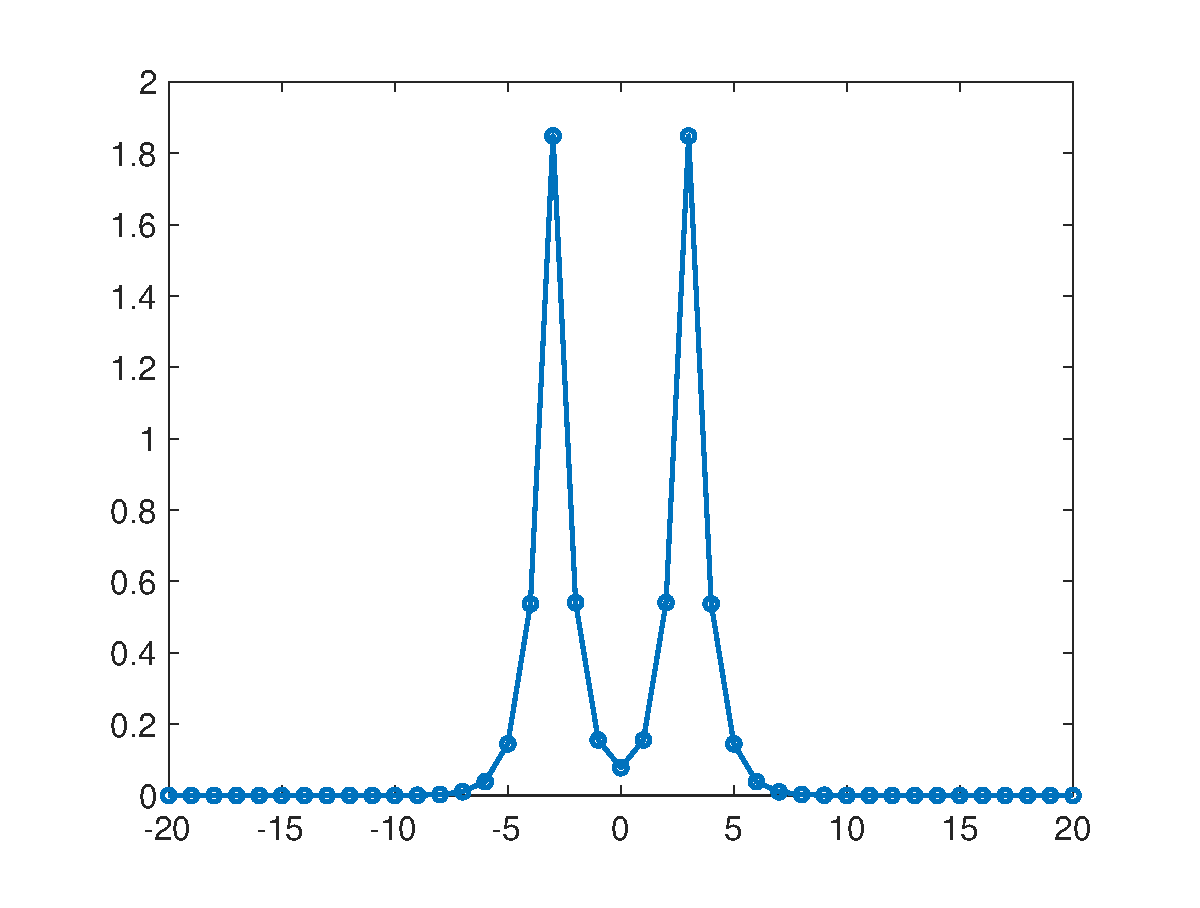
\includegraphics[width=5cm]{dnlsPP.eps}
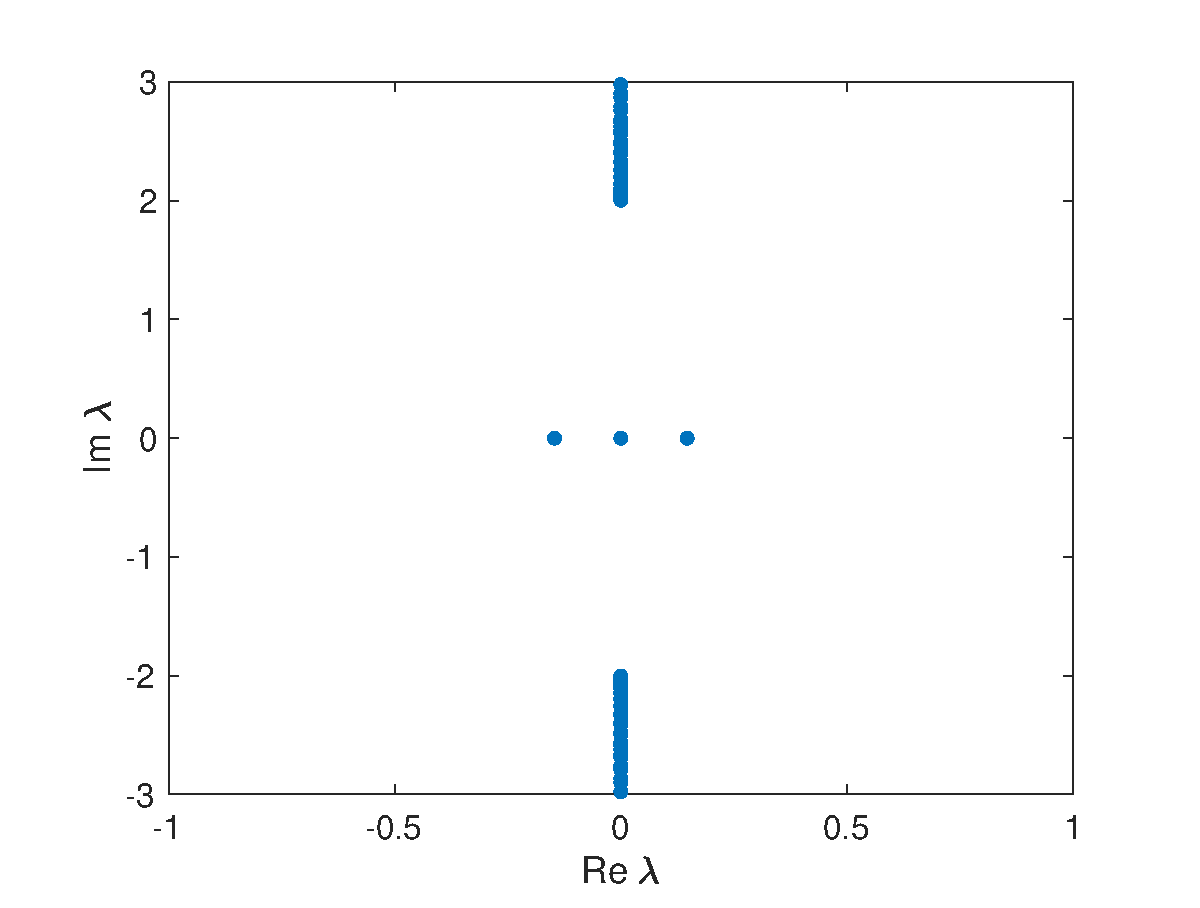
\includegraphics[width=5cm]{dnlsPPeig.eps}
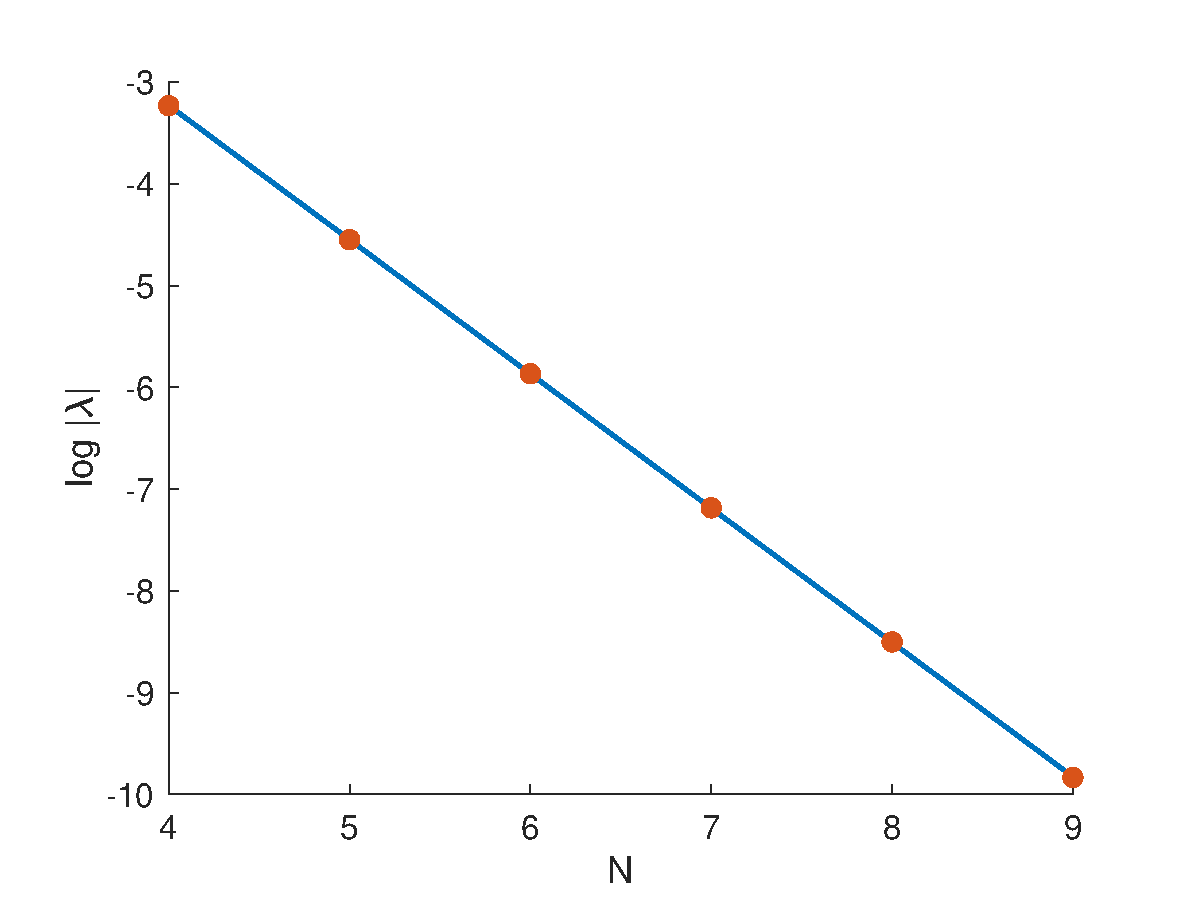
\includegraphics[width=5cm]{dnlsPPdecay.eps}
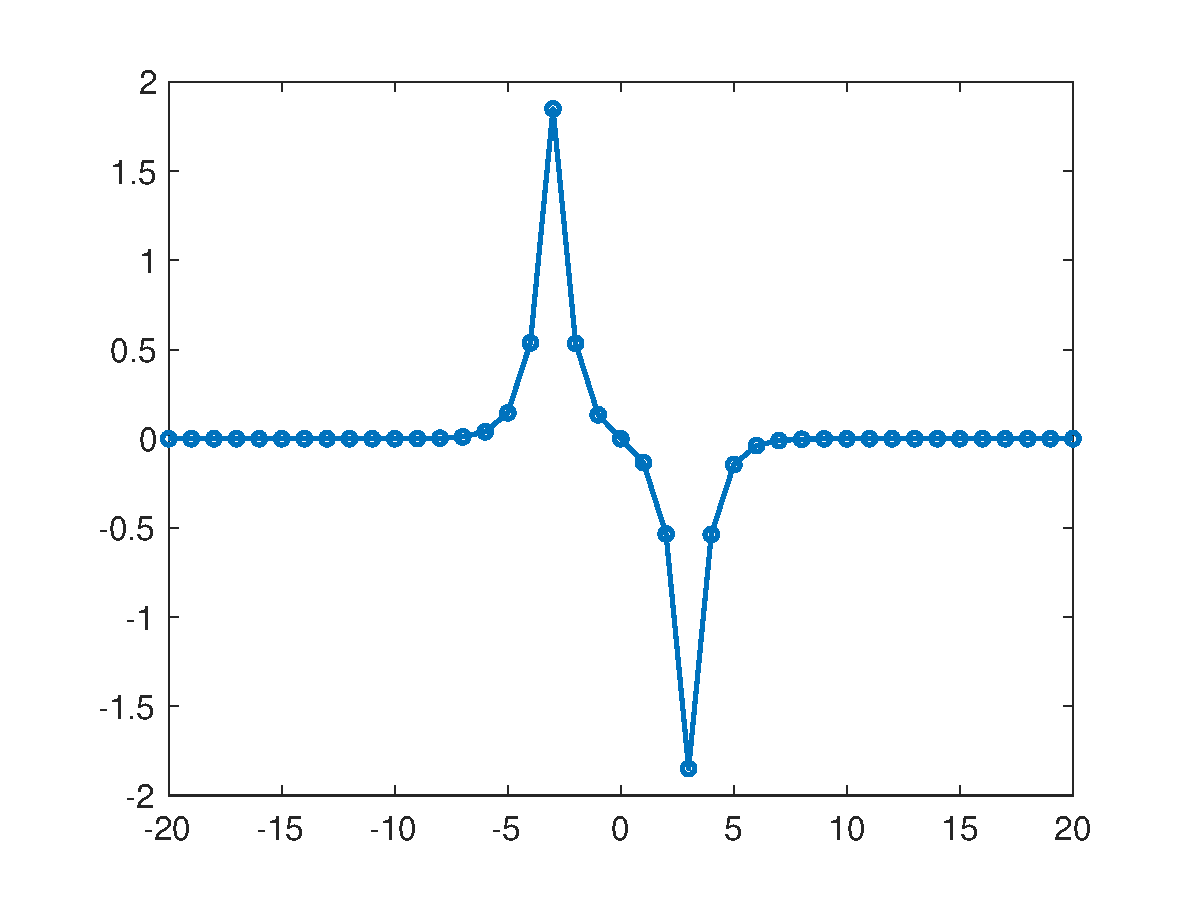
\includegraphics[width=5cm]{dnlsPM.eps}
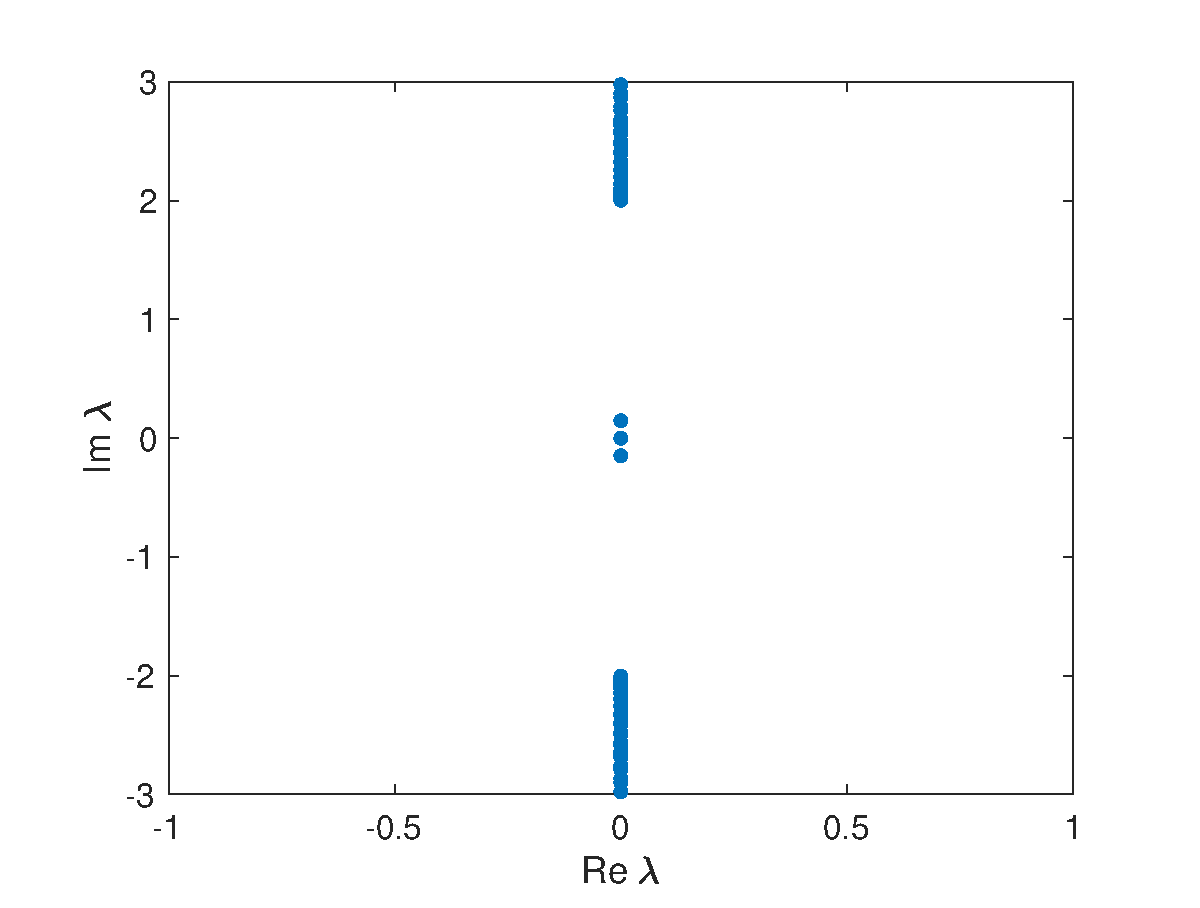
\includegraphics[width=5cm]{dnlsPMeig.eps}
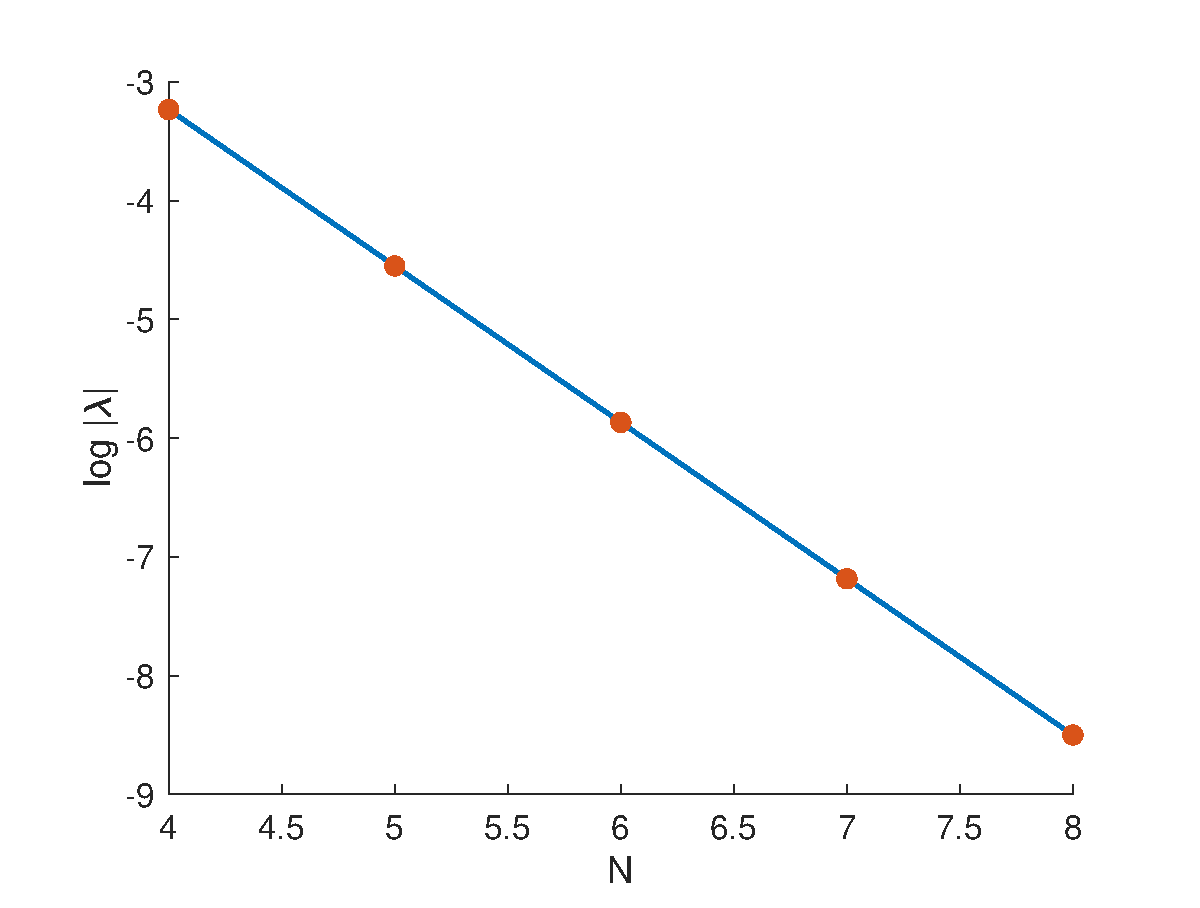
\includegraphics[width=5cm]{dnlsPMdecay.eps}
\label{fig:eigendecay1}
\caption{Solution, eigenvalue pattern, and plot of $\log(\lambda)$ vs. $N$ for $++$ (top) and $+-$ (bottom) solitons. Parameters $\omega = 2$ and $\epsilon = 1.0$}
\end{figure}
In both cases, the relative error in the eigenvalue decay rate from that predicted by the theory is order $1e-4$.

\begin{figure}[H]
\centering
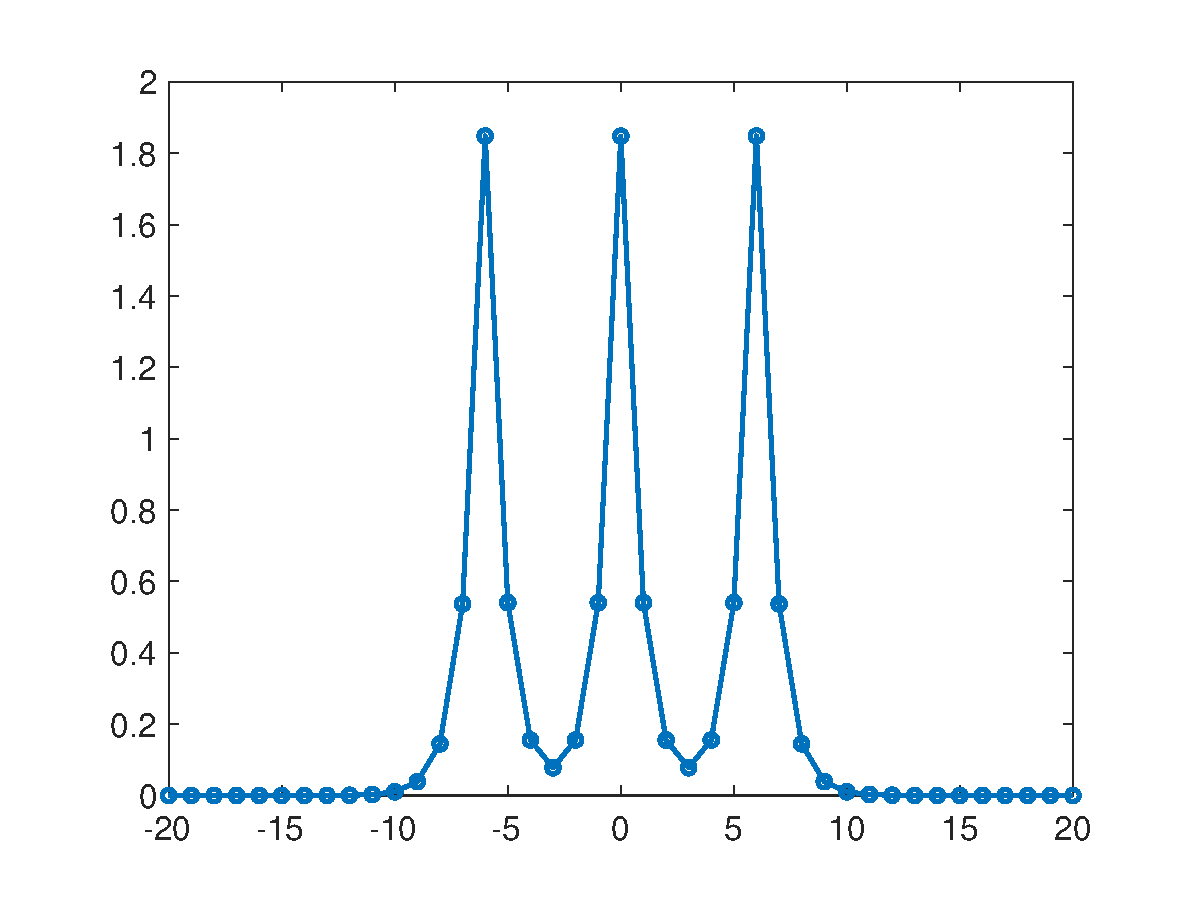
\includegraphics[width=5cm]{dnlsPPP.eps}
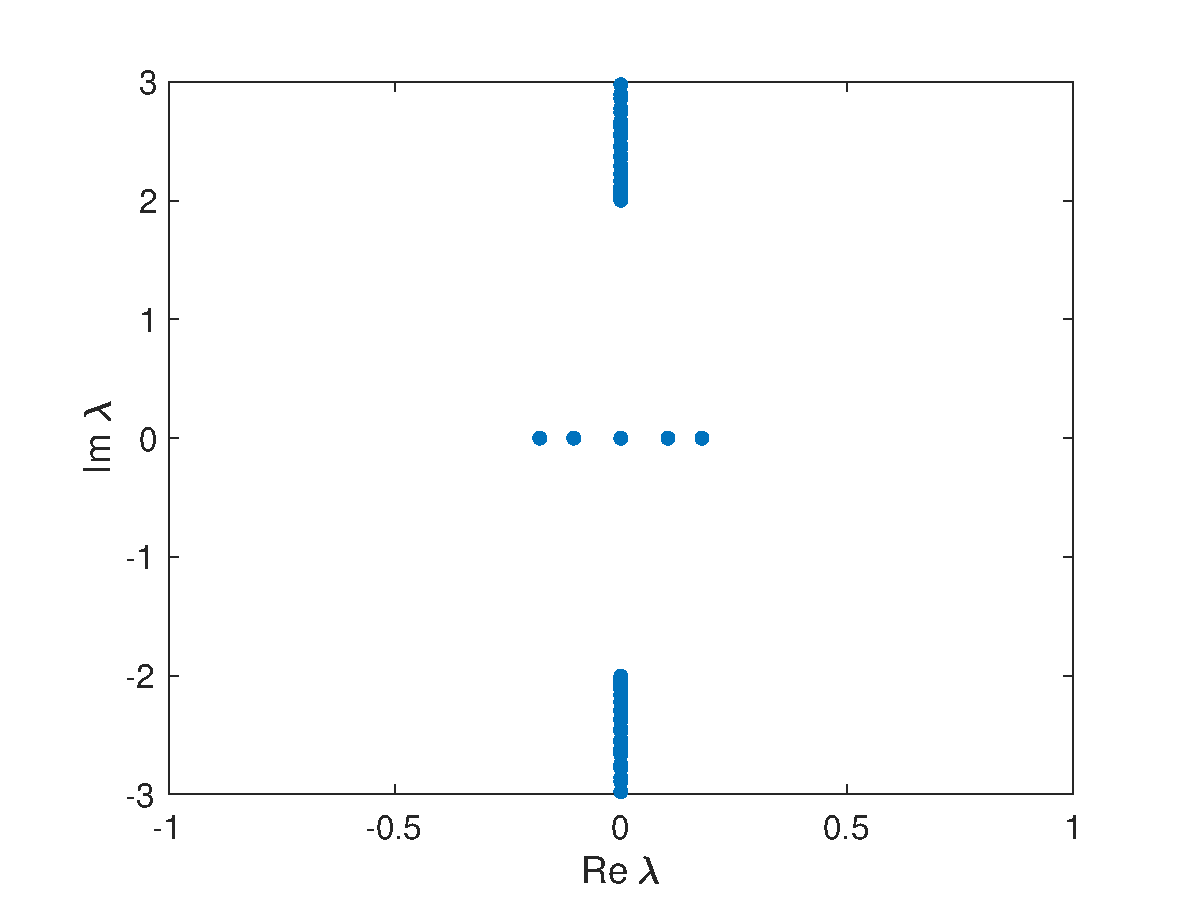
\includegraphics[width=5cm]{dnlsPPPeig.eps}
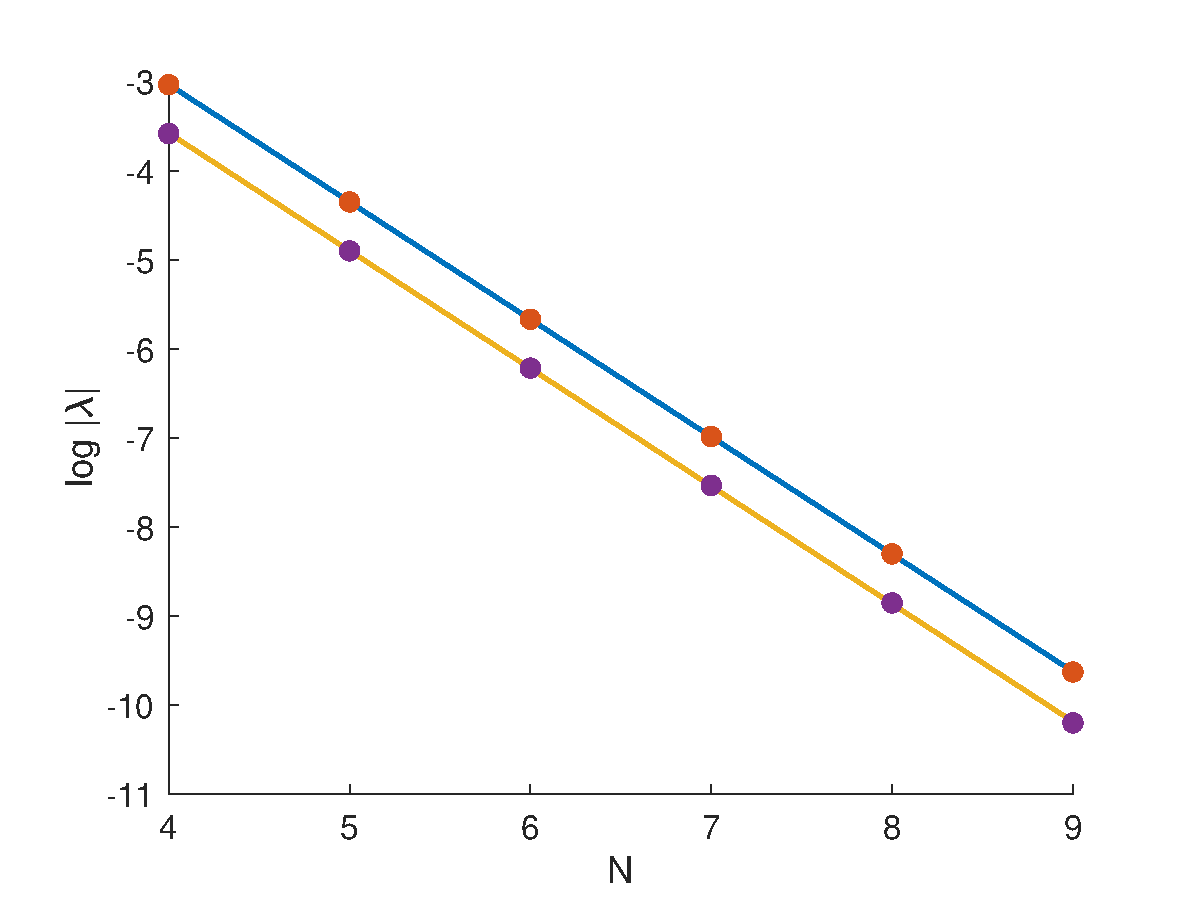
\includegraphics[width=5cm]{dnlsPPPdecay.eps}
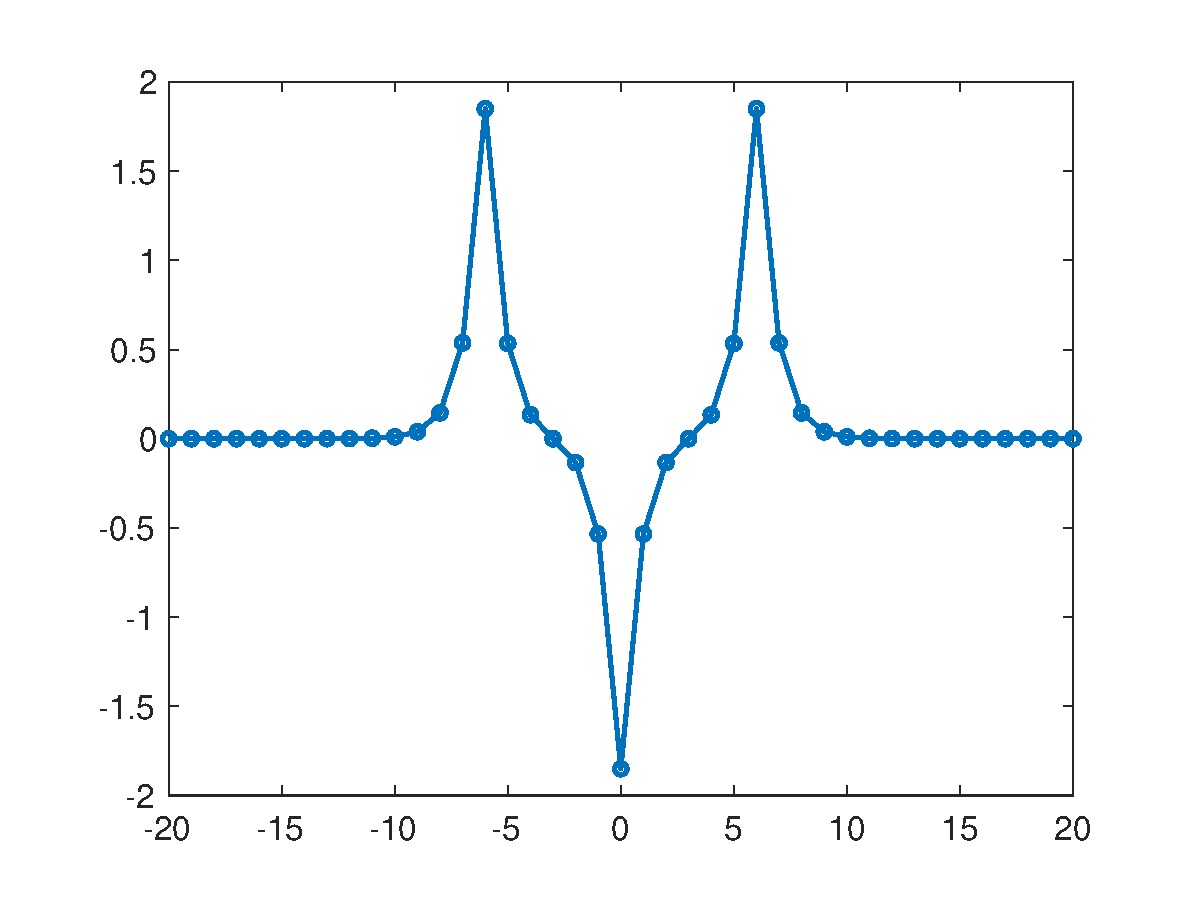
\includegraphics[width=5cm]{dnlsPMP.eps}
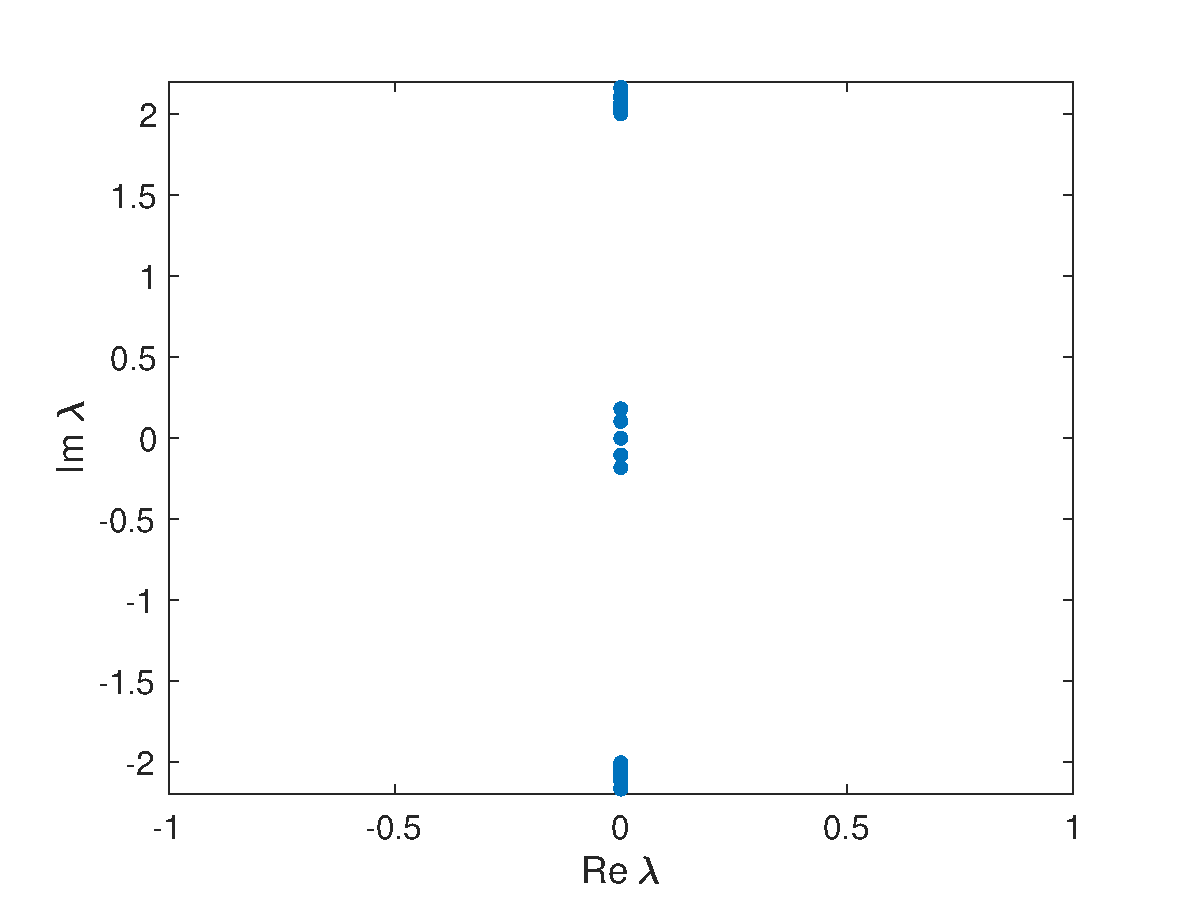
\includegraphics[width=5cm]{dnlsPMPeig.eps}
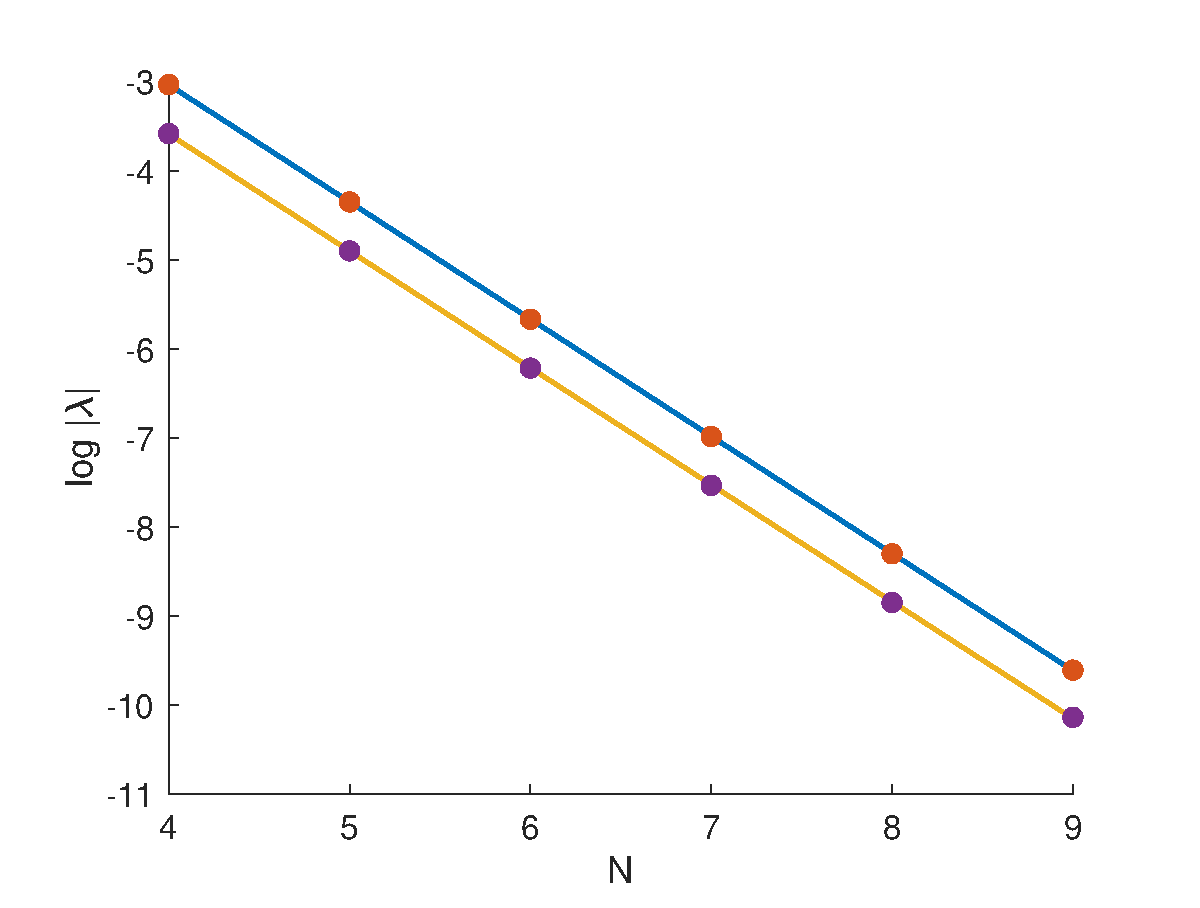
\includegraphics[width=5cm]{dnlsPMPdecay.eps}
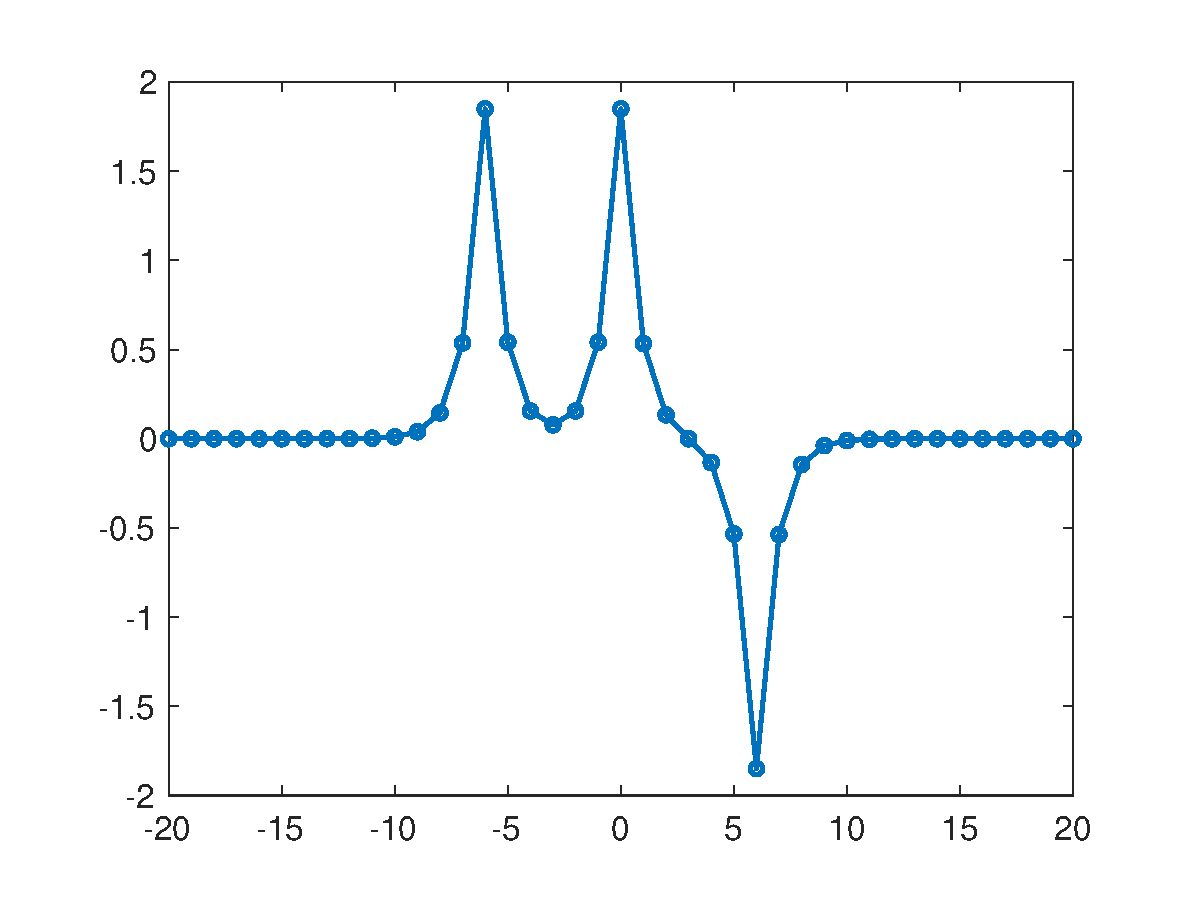
\includegraphics[width=5cm]{dnlsPPM.eps}
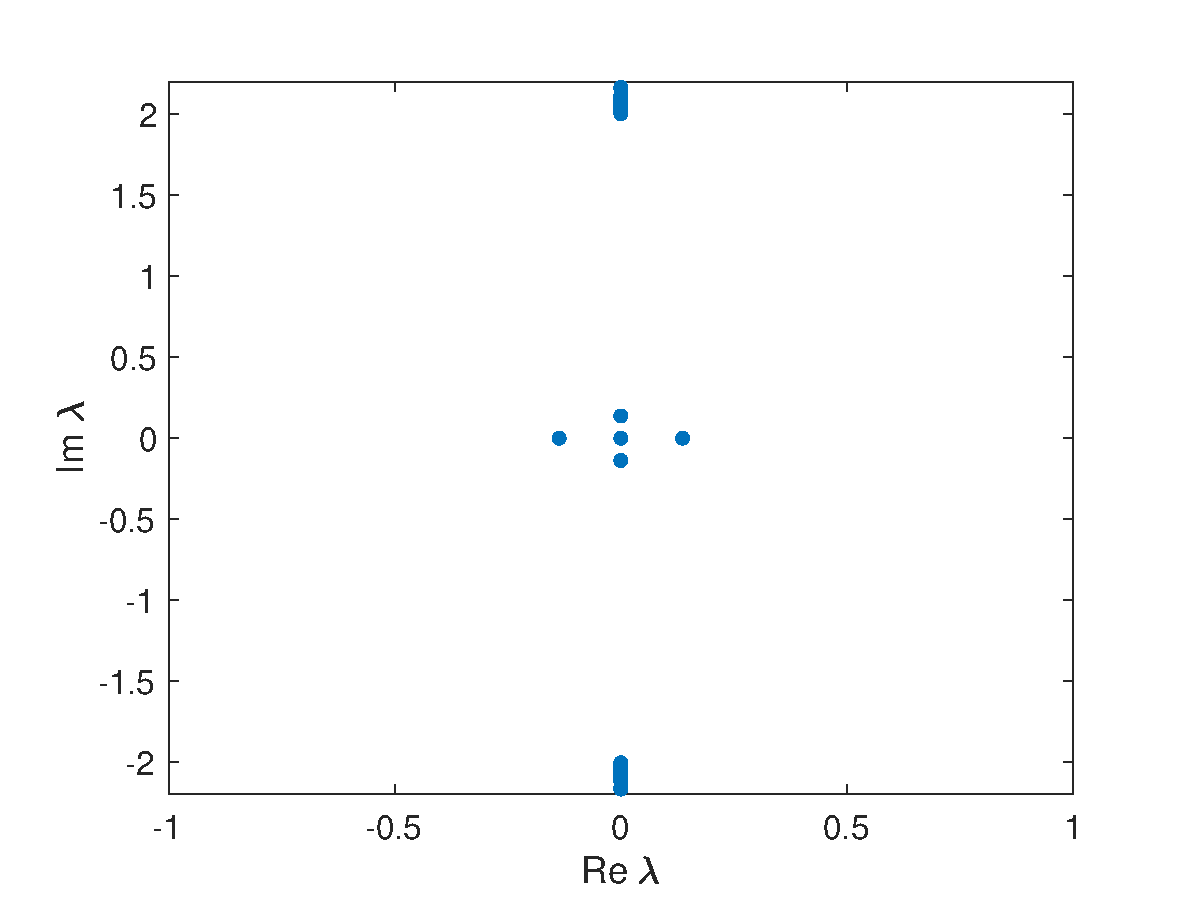
\includegraphics[width=5cm]{dnlsPPMeig.eps}
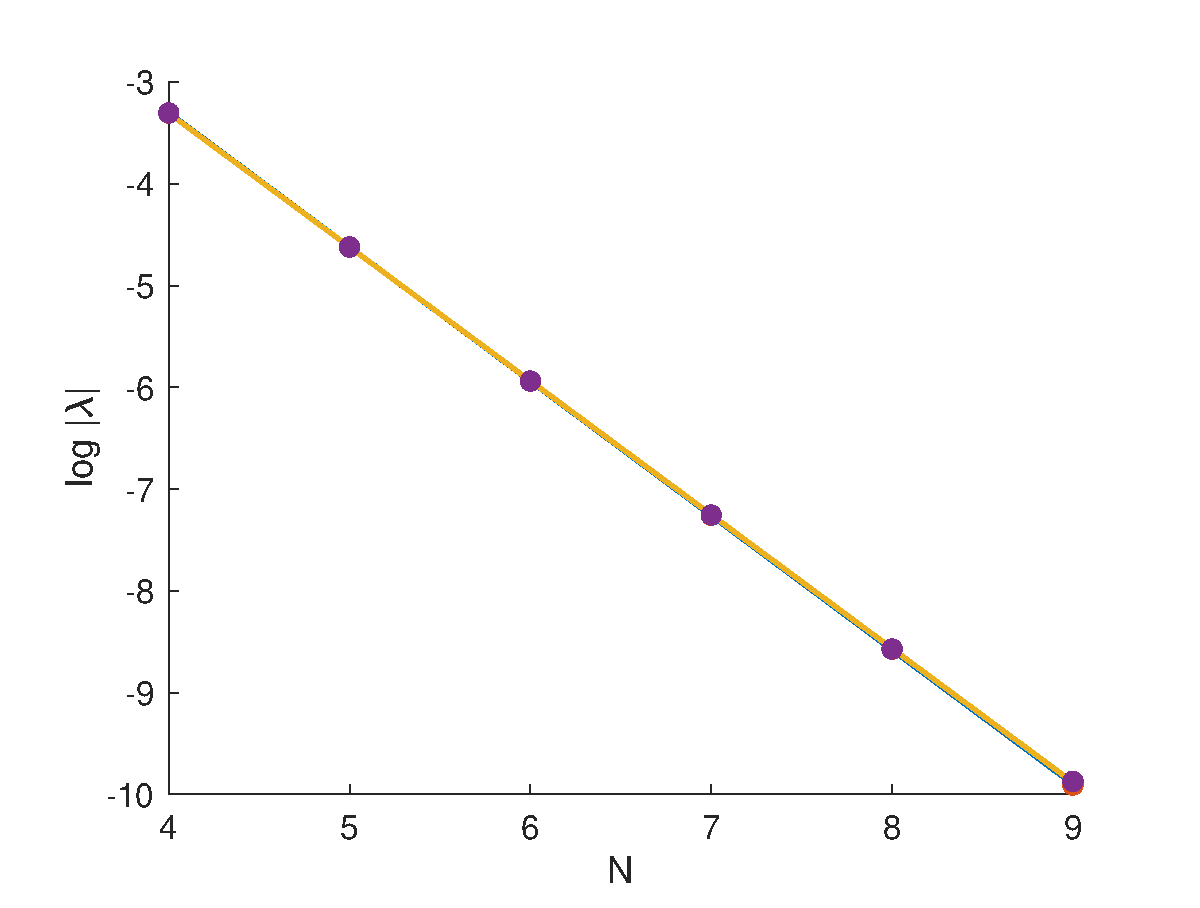
\includegraphics[width=5cm]{dnlsPPMdecay.eps}
\label{fig:eigendecay2}
\caption{Solution, eigenvalue pattern, and plot of $\log(\lambda)$ vs. $N$ for $+++$ (top), $+-+$ (middle), and $++-$ solitons. Parameters $\omega = 2$ and $\epsilon = 1.0$}
\end{figure}

\section{Proof of Existence Theorems}

\subsection{Discrete Exponential Dichotomy}

First, we define the discrete evolution operator for linear difference equations.

% lemma : discrete evolution operator
\begin{lemma}[Discrete Evolution Operator]\label{evolop}
Consider the difference equation together with its adjoint
\begin{align}
V(n+1) &= A(n) V(n) \label{diffeqevol} \\
Z(n+1) &= [A(n)^{-1}]^* Z(n) \label{adjeqevol}
\end{align}
where $n \in \Z$, $V(n) \in R^d$, and the matrix $A(n)$ is invertible for all $n$. Define the discrete evolution operator by
\begin{equation}\label{evol}
\Phi(m, n) = 
\begin{cases}
I & m = n \\
A(m-1) \dots A(n+1) A(n) & m > n \\
A^{-1}(m) \dots A^{-1}(n-2) A^{-1}(n-1) & m < n
\end{cases}
\end{equation}
\begin{enumerate}[(i)]
\item The evolution operators $\Phi$ of \eqref{diffeqevol} and $\Psi$ of \eqref{adjeqevol} are related by
\begin{equation}\label{adjevol}
\Psi(m, n) = \Phi(n, m)^*
\end{equation}
\item If $V(n)$ is a solution to \eqref{diffeqevol} and $Z(n)$ is a solution to \eqref{adjeqevol}, then the inner product $\langle V(n), Z(n) \rangle$ is constant in $n$.
\end{enumerate}

\begin{proof}
For (i), the result holds trivially for $m = n$. For, $m < n$ we have
\begin{align*}
\Psi(m, n) &= A(m)^* \dots A(n-2)^* A(n-1)^* \\
&= [A(n-1) A(n-2) \dots A(m)]^* \\
&= \Phi(n, m)^*
\end{align*}
The case for $m > n$ is similar.

For (ii), we have
\begin{align*}
\langle V(n+1), Z(n+1) \rangle &= 
\langle A(n) V(n), [A(n)^{-1}]^* Z(n) \rangle \\
&= \langle A(n)^{-1} A(n) V(n), Z(n) \rangle \\
&= \langle V(n), Z(n) \rangle
\end{align*}
\end{proof}
\end{lemma}

Next, we give a criterion for an exponential dichotomy.

% lemma : exp dichotomy in discrete case
\begin{lemma}[Exponential Dichotomy]\label{dichotomy}
Consider the difference equation
\begin{equation}\label{diffeqdichot}
V(n+1) = A(n) V(n)
\end{equation}
Suppose there exists a constant $0 < r < 1$ and a constant coefficient matrix $A$ such that 
\begin{equation}\label{Anexpdecay}
|A(n) - A| \leq C r^{|n|}
\end{equation}
and $|\lambda| \leq r$ or $|\lambda_\pm| \geq 1/r$ for all eigenvalues $\lambda$ of $A$. Then \eqref{diffeqdichot} has exponential dichotomies on $Z^\pm$. Specifically, there exist projections $P_\pm^s$ and $P_\pm^u$ defined on $\Z^\pm$ such that the following are true.
\begin{enumerate}[(i)]
\item
\begin{equation}\label{projcommute}
P_\pm^{s/u}(m) \Phi(m, n) =  \Phi(m, n) P_\pm^{s/u}(n)
\end{equation}

\item Let $\Phi_\pm^{s/u}(m, n) = \Phi(m, n) P_\pm^{s/u}(n)$ for $m, n \geq 0$ and $m, n \leq 0$ (respectively). Then we have the estimates
\begin{align*}
|\Phi_+^s(m, n)| \leq C r^{m - n} && 0 \leq n \leq m \\
|\Phi_+^u(m, n)| \leq C r^{n - m} && 0 \leq m \leq n \\
|\Phi_-^s(m, n)| \leq C r^{m - n} && n \leq m \leq 0 \\
|\Phi_-^u(m, n)| \leq C r^{n - m} && m \leq n \leq 0
\end{align*}
where the evolution operator $\Phi(m, n)$ is defined in Lemma \ref{evolop}. 

\item Let $E_\pm^{s/u}$ be the stable and unstable eigenspaces of $A^\pm$ and $Q_\pm^{s/u}$ the corresponding eigenprojections. Then we have
\begin{align*}
\dim \text{range }P_\pm^s(n) &= \dim E_\pm^s \\
\dim \text{range }P_\pm^u(n) &= \dim E_\pm^u
\end{align*}
and the exponential decay rates
\begin{align}\label{projexpdecay}
| P_\pm^{s/u}(n) - Q_\pm^{s/u} | \leq C r^{|n|}
\end{align}
\end{enumerate}

\begin{proof}
We will consider the problem on $\Z^+$. Since $A$ is constant coefficient and hyperbolic, the difference equation $W(n+1) = A^+ W(n)$ has an exponential dichotomy on $\R^+$. All the results except for \eqref{projexpdecay} follow directly from \cite[Proposition 2.5]{Beyn1997}. Equation \eqref{projexpdecay} follows from using the estimate \eqref{Anexpdecay} in the proof of \cite[Proposition 2.5]{Beyn1997}.
\end{proof}
\end{lemma}

The last thing we will need is a version of the variation of constants formula for the discrete setting.

\begin{lemma}[Variation of Constants Formula]\label{VOC}
For the initial value problem
\begin{align*}
V(n+1) &= A(n) V(n) + G(V(n), n) \\
V(n_0) &= V_{n_0}
\end{align*}
the solution $V(n)$ can be written as 
\begin{equation}\label{VOCformula}
V(n) = 
\begin{cases}
V_{n_0} & n = n_0 \\
\Phi(n, n_0) V_{n_0} + \sum_{j = n_0}^{n-1} \Phi(n, j+1) G(V(j), j)) & n > n_0 \\
\Phi(n, n_0) V_{n_0} - \sum_{j = n}^{n_0-1} \Phi(n, j+1) G(V(j), j)) & n < n_0 
\end{cases}
\end{equation}
\begin{proof}
For $n = n_0 + 1$,
\[
V(n_0 + 1) = A(n_0) V(n_0) + G(V(n_0), n_0) = \Phi(n_0+1, n_0) V(_0) + \Phi(n_0, n_0) G(V(n_0), n_0)
\]
Iterate this to get the result for $n > n_0$. The case for $n < n_0$ is similar.
\end{proof}
\end{lemma}

\subsection{Fixed Point Formulation}

Let $\Phi(m, n; \theta)$ be the evolution operator for
\begin{equation}\label{Vtheta}
V(n+1; \theta) = T(\theta) D_U F(Q(n)) T(\theta)^{-1} V(n; \theta) 
\end{equation}
Using \eqref{DFtheta} and the definition of the evolution operator \eqref{evol},
\[
\Phi(m, n; \theta) = T(\theta)\Phi(m, n; 0)T(\theta)^{-1}
\]

Furthermore, since $T(\theta) D_U F(Q(n)) T(\theta)^{-1}$ decays exponentially to $T(\theta) D_U F(0) T(\theta)^{-1}$ and $D_U F(0)$ is hyperbolic by Hypothesis \ref{initialhyp}(i), equation \eqref{Vtheta} has exponential dichotomies on $\Z^+$ and $\Z^-$ by Lemma \ref{dichotomy}. Let $P_{s/u}^\pm(m; \theta)$ and $\Phi_{s/u}^\pm(m, n; \theta)$ be the projections and evolutions of this exponential dichotomy for the ODE \ref{Vtheta}. The projections $P_{s/u}^\pm(m; \theta)$ are related to those for $\theta = 0$ by
\[
P_{s/u}^\pm(m; \theta) = T(\theta)P_{s/u}^\pm(m; 0)T(\theta)^{-1}
\]
Finally, let $E^s(\theta)$ and $E^u(\theta)$ be the stable and unstable eigenspaces of $T(\theta) D_U F(0) T(\theta)^{-1}$, and let $P_0^s(\theta)$ and $P_0^u(\theta)$ be the corresponding eigenprojections.

We note that the estimates from Lemma \ref{dichotomy} do not depend on $\theta$. Finally, if we take Hypothesis \ref{intersectionhyp}(ii), $T'(0) Q(n)$ is a solution to \eqref{Vtheta}.

Next, as in \cite{Sandstede1997} and \cite{Knobloch2000}, we write equation \eqref{Wsystem1} in fixed-point form using the discrete variation of constants formula from Lemma \ref{VOCformula} together with projections on the stable and unstable subspaces of the exponential dichotomy.
\begin{equation}\label{FPeqs1}
\begin{aligned}
W_i^-(n) &= 
\Phi_s^-(n, -N_{i-1}^-; \theta_i) a_{i-1}^- + \Phi_u^-(n, 0; \theta_i) b_i^-  \\
&+ \sum_{j = -N_{i-1}^-}^{n-1} \Phi_s^-(n, j+1; \theta_i) G_i^-(W_i^-(j)) - \sum_{j = n}^{-1} \Phi_u^-(n, j+1; \theta_i) G_i^-(W_i^-(j)) \\
W_i^+(n) &= \Phi_u^+(n, N_i^+; \theta_i) a_i^+ + \Phi_s^+(n, 0; \theta_i) b_i^+ \\
&+ \sum_{j = 0}^{n-1} \Phi_s^+(n, j+1; \theta_i) G_i^+(W_i^+(j)) 
- \sum_{j = n}^{N_i^+-1} \Phi_u^+(n, j+1; \theta_i) G_i^+(W_i^+(j))
\end{aligned}
\end{equation}
where $W_i^-(n) \in l^\infty([-N_{i-1}^-, 0])$, $W_i^+(n) \in l^\infty([0, N_i^+])$, and the sums are defined to be $0$ if the upper index is smaller than the lower index. For the initial conditions, we have
\begin{enumerate}
\item $a_i^- \in E^s(\theta_i)$, $a_i^+ \in E^u(\theta_i)$, and $a_0^- = a_m^+ = 0$
\item $b_i^+ \in T(\theta_i) Y^+$ and $b_i^- \in T(\theta_i) Y^-$.
\end{enumerate}
We note that if Hypothesis \ref{intersectionhyp}(ii) holds, we do not need to include a component in $T'(0) Q(0)$ in $b_i^\pm$, since that direction is handled by the symmetry parameter $\theta_i$.

Since we wish to construct a homoclinic orbit to the rest state at 0, we take the initial conditions $a_0^- = 0$ and $a_m^+ = 0$. For these cases, the fixed point equations are given by
\begin{align*}
W_1^-(n) &= \Phi_u^-(n, 0; \theta_i) b_i^- 
+ \sum_{j = -\infty}^{n-1} \Phi_s^-(n, j+1; \theta_i) G_i^-(W_i^-(j)) - \sum_{j = n}^{-1} \Phi_u^-(n, j+1; \theta_i) G_i^-(W_i^-(j)) \\
W_m^+(n) &= \Phi_s^+(n, 0; \theta_i) b_i^+ 
+ \sum_{j = 0}^{n-1} \Phi_s^+(n, j+1; \theta_i) G_i^+(W_i^+(j)) 
- \sum_{j = n}^\infty \Phi_u^+(n, j+1; \theta_i) G_i^+(W_i^+(j))
\end{align*}
where the infinite sums converge due to the exponential dichotomy. 

\subsection{Inversion}

As in \cite{Sandstede1997}, we will solve equations \eqref{Wsystem1}, \eqref{Wsystem2}, and \eqref{Wsystem3} in stages. The first two steps are the same regardless of whether we take Hypothesis \ref{intersectionhyp}(i) or \ref{intersectionhyp}(ii). In the first lemma of this section, we solve for $W_i^\pm$. 

% solve for W
\begin{lemma}\label{inv1}
There exist unique bounded functions $W_i^\pm(n)$ such that equation \eqref{Wsystem1} is satisfied. These solutions depend smoothly on the initial conditions $a_i^\pm$ and $b_i\pm$, and we have the estimates.
\begin{equation}\label{Wipmest}
\begin{aligned}
||W_i^-|| &\leq C (|a_{i-1}^-| + |b_i^-|) \\
||W_i^+|| &\leq C (|a_i^+| + |b_i^+| )
\end{aligned}
\end{equation}
For the interior pieces, we have the piecewise estimates
\begin{equation}\label{Wipiecewise}
\begin{aligned}
|W_i^-(n)| &\leq C (r^{-(N_{i-1}^- + n)}|a_{i-1}^-| + r^n|b_i^-|) && n \in [-N_{i-1}^-, 0] \\
|W_i^+(n)| &\leq C (r^{-(N_i^+ - n)}|a_i^+| + r^{-n}|b_i^+| ) && n \in [0, N_i^+] 
\end{aligned}
\end{equation}

\begin{proof}
First, we show that the RHS of the fixed point equations \eqref{FPeqs1} defines a smooth map from $l^\infty$ (on the appropriate interval) to itself. For the $W_i^-$, we have
\begin{align}\label{inv1est1}
|\Phi_s^-(n, &-N_{i-1}^-; \theta_i) a_{i-1}^-| + |\Phi_u^-(n, 0; \theta_i) b_i^-| \leq C ( |a_{i-1}^-| + |b_i^-|) 
\end{align}
and
\begin{align*}
\left| \sum_{j = -N_{i-1}^-}^{n-1} \Phi_s^-(n, j+1; \theta_i) G_i^-(W_i^-(j))\right| + \left|\sum_{j = n}^{-1} \Phi_u^-(n, j+1; \theta_i) G_i^-(W_i^-(j))\right| 
\leq C ||W_i^-||_{l^\infty([-N_{i-1}, 0])}^2 
\end{align*}
both of which are independent of $n$. Define the map $H_i^-: l^\infty([-N_{i-1}, 0]) \times E^s \times Y^- \rightarrow l^\infty([-N_{i-1}, 0])$ by
\begin{align}\label{inv1map}
H_i^-(W_i^-(n), &a_{i-1}^-, b_i^-) = W_i^-(n) - \Phi_s^-(n, -N_{i-1}^-; \theta_i) a_{i-1}^- - \Phi_u^-(n, 0; \theta_i) b_i^-  \\
&- \sum_{j = -N_{i-1}^-}^{n-1} \Phi_s^-(n, j+1; \theta_i) G_i^-(W_i^-(j)) + \sum_{j = n}^{-1} \Phi_u^-(n, j+1; \theta_i) G_i^-(W_i^-(j)) \nonumber
\end{align}
Since 0 is an equilibrium, $H(0, 0, 0) = 0$. It is not hard to show that the Fr\'echet derivative of $H_i^-$ with respect to $W_i^-$ at $(W_i^-(n), a_{i-1}^-, b_i^-) = (0, 0, 0)$ is a Banach space isomorphism on $l^\infty([-N_{i-1}, 0])$. Thus we can solve for $W_i^-(x)$ in terms of $(a_{i-1}^-, b_i^-)$ using the IFT. This dependence is smooth, since the map $H_i^-$ is smooth. The estimate \eqref{Wipmest} on $W_i^-$ comes from \eqref{inv1est1}, since the terms in \eqref{inv1map} involving sums are quadratic in $W_i^\pm$. The case for $W_i^+$ is similar. Finally, for the interior pieces, we can easily obtain the piecewise estimates \eqref{Wipiecewise}.
\end{proof}
\end{lemma}

Next, we use the center matching conditions at $N_i^\pm$ to solve for the initial conditions $a_i^\pm$.

% match in middles
\begin{lemma}\label{inv2}
For $i = 1, \dots m-1$ there is a unique pair of initial conditions $(a_i^+, a_i^-) \in E^u(\theta_i) \times E^s(
\theta_i)$ such that the matching conditions \eqref{Wsystem2} are satisfied. $(a_i^+, a_i^-)$ depends smoothly on $(b_i^+, b_{i+1}^-)$, and we have the following expressions for $a_i^-$ and $a_i^+$. 
\begin{equation}\label{aipmest}
\begin{aligned}
a_i^+ &= P_0^u(\theta_i) d_i + \tilde{a}_i^+ \\
a_i^- &= -P_0^s(\theta_i) d_i + \tilde{a}_i^-
\end{aligned}
\end{equation}
where 
\begin{equation}\label{tildeaest}
\tilde{a}_i^\pm = \mathcal{O}(r^{-N}(|b_i^+|+|b_{i+1}^-|) + |b_i^+|^2+|b_{i+1}^-|^2) 
\end{equation}
In terms of $Q(\pm N_i^\pm)$, we can write \eqref{aipmest} as 
\begin{equation}\label{aipmexp}
\begin{aligned}
a_i^- &= T(\theta_i) Q(N_i^+) + \tilde{a}_i^- + \mathcal{O}(r^{-2N}) \\
a_i^+ &= T(\theta_{i+1}) Q(-N_i^-) + \tilde{a}_i^+ + \mathcal{O}(r^{-2N})
\end{aligned}
\end{equation}

\begin{proof}
Evaluating the fixed point equations \eqref{FPeqs1} at $\pm N_i^\pm$ and subtracting, solving equation \eqref{Wsystem2} is equivalent to solving $H_i(a_i^+, a_i^-, b_i^+, b_{i+1}^-) = 0$, where $H_i: E^s \times E^u \times Y^+ \times Y^- \times \rightarrow \R^d$ is defined by
\begin{align*}
H_i(a_i^+, &a_i^-, b_i^+, b_{i+1}^-) \\
&= a_i^+ - a_i^- - d_i + (P_u^+(N_i^+; \theta_i) - P_0^u) a_i^+ - (P_s^-(-N_i^-; \theta_{i+1}) - P_0^s) a_i^- \\
&+ \Phi_s^+(N_i^+, 0; \theta_i) b_i^+ - \Phi_u^-(-N_i^-, 0; \theta_{i+1}) b_{i+1}^- \\
&+ \sum_{j = 0}^{N_i^+-1} \Phi_s^+(N_i^+, j+1; \theta_i) G_i^+(W_i^+(j; a_i^+, b_i^+)) \\
&+ \sum_{j = -N_i^-}^{-1} \Phi_u^-(-N_i^-, j+1; \theta_{i+1}) G_i^-(W_{i+1}^-(j; a_i^-, b_{i+1}^-))
\end{align*}
and we substituted $W_{i+1}^-(n; a_i^-, b_{i+1}^-)$ and $W_i^+(n; a_i^+, b_i^+)$ from Lemma \ref{inv1}. Next, we note that $H_i(0,0,0,0) = 0$ and that 
\begin{align*}
\frac{\partial}{\partial a_i^-} H_i(0, 0, 0, 0) &= -1 + \mathcal{O}(r^{-N_i^-}) \\
\frac{\partial}{\partial a_i^+} H_i(0, 0, 0, 0) &= 1 + \mathcal{O}(r^{-N_i^+})
\end{align*}
since the derivatives of the terms in $H_i$ involving sums will be 0 since $G_i^\pm$ is quadratic in $W_i^\pm$, thus quadratic order in $a_i^\pm$ by Lemma \ref{inv1}. For sufficiently large $N$, $D_{a_i^\pm} H(0, 0, 0, 0, 0)$ is invertible in a neighborhood of $(0, 0, 0, 0, 0)$. Thus, since $(a_i^+, a_i^-) \in E^s(\theta_i) \oplus E^u(\theta_i) = \R^d$, we can use the IFT to solve for $a_i^\pm$ in terms of $(b_i^+$, $b_{i+1}^-)$ for $(b_i^+, b_{i+1}^-)$ sufficiently small.

To get the estimates on and expressions for $a_i^\pm$, we project $H_i(a_i^+, a_i^-, b_i^+, b_{i+1}^-) = 0$ onto $E^s(\theta_i)$ and $E^u(\theta_i)$ in turn to get 
\begin{align*}
a_i^+ &= P_0^u(\theta_i) d_i + \mathcal{O}(r^{-N}(|b_i^+|+|b_{i+1}^-|) + |b_i^+|^2+|b_{i+1}^-|^2) \\
a_i^- &= -P_0^s(\theta_i) d_i + \mathcal{O}(r^{-N}(|b_i^+|+|b_{i+1}^-|) + |b_i^+|^2+|b_{i+1}^-|^2)
\end{align*}
which we can write in the form \eqref{aipmest} with estimates \eqref{tildeaest}. 

To write these in terms of $Q(\pm N_i^\pm)$, we note that
\begin{align*}
P_0^s(\theta_i) T(\theta_i) Q(N_i^+) &= (P_0^s(\theta_i) - P_s^+(N_i^+; \theta_i)) T(\theta_i) Q(N_i^+) + P_s^+(N_i^+; \theta_i) T(\theta_i) Q(N_i^+) \\
&= T(\theta_i)(P_0^s(0) - P_s^+(N_i^+; 0)) Q(N_i^+) + P_s^+(N_i^+; \theta_i) T(\theta_i) Q(N_i^+) \\
&= T(\theta_i) Q(N_i^+) + \mathcal{O}(r^{-2N}) 
\end{align*}
where in the second line we used \eqref{projexpdecay}. Similarly, we can show that 
\begin{align*}
P_0^s T(\theta_{i+1}) Q(-N_i^-) &= \mathcal{O}(r^{-2N})
\end{align*}
Substituting these into \eqref{aipmest} we obtain \eqref{aipmexp}.
\end{proof}
\end{lemma}

It only remains to satisfy \eqref{Wsystem3}. At this point, we have to treat the two cases for \ref{intersectionhyp} separately.

First, we consider the transverse intersection case. If  Hypothesis \ref{intersectionhyp}(i) holds, existence of the multi-pulse solutions follows from the implicit function theorem as long as $N$ is sufficiently large.

% center match, transverse intersection
\begin{lemma}\label{inv3t}
Assume Hypothesis \ref{intersectionhyp}(i). Then for $i = 1, \dots m$ there is a unique pair of initial conditions $(b_i^-, b_i^+) \in T(\theta_i) Y^- \times T(\theta_i) Y^+$ such that the matching conditions \eqref{Wsystem3} are satisfied. We have the uniform bound
\begin{equation}\label{bboundt}
b = \mathcal{O}(r^{-2N})
\end{equation}

\begin{proof}
Evaluating the fixed point equations \eqref{FPeqs1} at 0 and subtracting, we have
\begin{align*}
W_i^+(0) &- W_i^-(0) = b_i^+ - b_i^- 
+ \Phi_u^+(0, N_i^+; \theta_i) a_i^+ - \Phi_s^-(0, -N_{i-1}^-; \theta_i) a_{i-1}^- \\
&- \sum_{j = 0}^{N_i^+-1} \Phi_u^+(0, j+1; \theta_i) G_i^+(W_i^+(j)) 
- \sum_{j = -N_{i-1}^-}^{-1} \Phi_s^-(0, j+1; \theta_i) G_i^-(W_i^-(j)) \\
\end{align*}
Next, substitute $W_i^\pm$ from Lemma \ref{inv1} and $a_i^\pm$ from Lemma \ref{inv2}. Define the spaces
\begin{align}\label{spaceYt}
Y &= \bigoplus_{i=1}^m (T(\theta) Y^+ \oplus T(\theta) Y^-) = \bigoplus_{i=1}^m \R^d \\
Z &= \bigoplus_{i=1}^{m-1} \R^d
\end{align}
Let $b = (b_1^+, b_1^-, \dots, b_m^+, b_m^-) \in Y$ and $d = (d_1, \dots, d_{m-1}) \in Z$. Define the function $H: Y \times Z \rightarrow Y$ component-wise by
\begin{align*}
H_i(b, d) &= 
 b_i^+ - b_i^- + \Phi_u^+(0, N_i^+; \theta_i) P_0^u d_i + \Phi_s^-(0, -N_{i-1}^-; \theta_i) P_0^s d_{i-1} \\
&+ \Phi_u^+(0, N_i^+; \theta_i) \tilde{a}_i^+(b_i^+, b_{i+1}^-) 
- \Phi_s^-(0, -N_{i-1}^-; \theta_i) \tilde{a}_{i-1}^-(b_{i-1}^+, b_i^-) \\
&- \sum_{j = 0}^{N_i^+-1} \Phi_u^+(0, j+1; \theta_i) G_i^+(W_i^+(j; b_i^+, b_{i+1}^-)) \\
&- \sum_{j = -N_{i-1}^-}^{-1} \Phi_s^-(0, j+1; \theta_i) G_i^-(W_i^-(j; b_{i-1}^+, b_i^-))
\end{align*}
where $d_0 = d_m = 0$, and we have indicated the dependencies on the $b_i^\pm$. Using the estimates from Lemmas \ref{inv1} and \ref{inv2}, $H(0, 0) = 0$. For the partial derivatives with respect to $b_i^\pm$, we have
\begin{align*}
\frac{\partial}{\partial b_i^+}H_i(0) &= 1 + \mathcal{O}(r^{-N})  \\
\frac{\partial}{\partial b_i^-}H_i(0) &= -1 + \mathcal{O}(r^{-N}) \\
\frac{\partial}{\partial b_{i-1}^+}H_i(0),
\frac{\partial}{\partial b_{i+1}^-}H_i(0) &= \mathcal{O}(r^{-N})
\end{align*}
For all other indices,
\[
\frac{\partial}{\partial b_j^\pm}H_i(0) = 0
\]
Thus, for sufficiently large $N$, the matrix $D_b H(0,0)$ is invertible. Using the IFT, there exists a unique smooth function $b: Z \rightarrow Y$ with $b(0) = 0$ such that $H(b(d),d) = 0$ for $d$ sufficiently small, which is the case for $N$ sufficiently large, since $d = \mathcal{O}(r^{-N})$.

The bound for $b$ comes from projecting $H_i(b(d), d) = 0$ onto $T(\theta)Y^+$ and $T(\theta)Y^-$ together with the estimate $d = \mathcal{O}(r^{-N})$.
\end{proof}
\end{lemma}

If Hypothesis \ref{intersectionhyp}(ii) holds, we will not in general be able to solve equation \eqref{Wsystem3}. Instead, we will obtain a set of jump conditions in the direction of $T(\theta) Z_1(0)$ which will depend on the symmetry parameters $\theta_i$. Satisfying the jump conditions can then be accomplished by adjusting the symmetry parameters.

Recall that for all $\theta \in \R$ we have the decomposition
\[
\R^d = \R T(\theta) T'(0)Q(0) \oplus T(\theta) Y^+ \oplus T(\theta) Y^- \oplus \R T(\theta) Z_1(0)
\]
Projecting in these directions, we can write \eqref{Wsystem3} as the system of equations
\begin{align}
P_{T(\theta)T'(0)Q(0)}\left( W_i^+(0) - W_i^-(0) \right) &= 0 \label{jumpS1} \\
P_{T(\theta)Y^+ \oplus T(\theta)Y^-}\left( W_i^+(0) - W_i^-(0) \right) &= 0 \label{jumpnonZ} \\
P_{\R T(\theta)Z_1(0)} \left( W_i^+(0) - W_i^-(0) \right) &= 0 \label{jumpZ}
\end{align}

Since $W_i^\pm(0) \in Y^+ \oplus Y^- \oplus \R Z_1(0)$, equation \ref{jumpS1} is automatically satisfied. Since $b_i^+ \in T(\theta) Y^+$ and $b_i^- \in T(\theta) Y^-$, we will be able to satisfy \eqref{jumpnonZ} by solving for the $b_i^\pm$, which we do in the following lemma.

% solve for $b_i^\pm$, nontransverse int
\begin{lemma}\label{inv3nt}
Assume Hypothesis \ref{intersectionhyp}(ii). Then for $i = 1, \dots m$ there is a unique pair of initial conditions $(b_i^-, b_i^+) \in T(\theta_i) Y^- \times T(\theta_i) Y^+$ such that the jump conditions \eqref{jumpnonZ} are satisfied. We have the uniform bound
\begin{equation}\label{bboundnt}
b = \mathcal{O}(r^{-2N})
\end{equation}
\begin{proof}
The proof is almost identical to that of Lemma \ref{inv3t}.
\end{proof}
\end{lemma}

Finally, we will look at equation \ref{jumpZ}. This condition will give us $m$ jump conditions in the direction of $T(\theta_i) Z_1$.

\begin{lemma}\label{jumpZlemma}
Assume Hypothesis \ref{intersectionhyp}(ii). Then the jump conditions in the direction of $T(\theta_i) Z_1$ are given by
\begin{equation*}
\begin{aligned}
\xi_1 &= \langle T(\theta_1) Z_1(N_1^+), T(\theta_2) Q(-N_1^-) \rangle + R_1  \\
\xi_i &= \langle T(\theta_i) Z_1(N_i^+), T(\theta_{i+1}) Q(-N_i^-) \rangle
- \langle T(\theta_i) Z_1(-N_{i-1}^-), T(\theta_{i-1}) Q(N_{i-1}^+) + R_i &&
i = 2, \dots, m-1 \\
\xi_m &= -\langle T(\theta_m) Z_1(-N_{m-1}^-), T(\theta_{m-1}) Q(N_{m-1}^+) + R_m
\end{aligned}
\end{equation*}
where the remainder term has bound
\begin{equation}\label{RZbound}
|R_i| \leq C r^{-3N}
\end{equation}
\begin{proof}
Evaluating the fixed point equations \eqref{FPeqs1} at 0 and substituting \eqref{aipmest} from Lemma \ref{inv1}, we get
\begin{align*}
W_i^+(0) &- W_i^-(0) = \Phi_u^+(0, N_i^+; \theta_i) P_0^u(\theta_i) d_i + \Phi_s^-(0, -N_{i-1}^-; \theta_i) P_0^s(\theta_{i-1}) d_{i-1} \\
&+ b_i^+ - b_i^- 
+ \Phi_u^+(0, N_i^+; \theta_i) \tilde{a}_i^+ - \Phi_s^-(0, -N_{i-1}^-; \theta_i) \tilde{a}_{i-1}^- \\
&- \sum_{j = 0}^{N_i^+-1} \Phi_u^+(0, j+1; \theta_i) G_i^+(W_i^+(j)) 
- \sum_{j = -N_{i-1}^-}^{-1} \Phi_s^-(0, j+1; \theta_i) G_i^-(W_i^-(j)) \\
\end{align*}
Next, we project on $\R T(\theta_i) Z_1(0)$ by taking the inner product with $T(\theta_i) Z_1(0)$. Since $b_i^\pm \in T(\theta_i) Y_i^\pm$, these terms are eliminated by the projection. For the leading order terms in \eqref{jumpZ}, using equation \eqref{didef} and the proof of Lemma \ref{inv2}, we have
\begin{align*}
\langle T(\theta_i) Z_1(0), \Phi_u^+(0, N_i^+; \theta_i) P_0^u d_i \rangle
&= \langle T(\theta_i) Z_1(N_i^+), T(\theta_{i+1}) Q(-N_i^-) \rangle + \mathcal{O}(r^{-3N}) \\
\langle T(\theta_i) Z_1(0), \Phi_s^-(0, -N_{i-1}^-; \theta_i) P_0^s d_{i-1} \rangle
&= -\langle T(\theta_i) Z_1(-N_{i-1}^-), T(\theta_{i-1}) Q(N_{i-1}^+) \rangle + \mathcal{O}(r^{-3N})
\end{align*}

For the higher order terms in \eqref{jumpZ}, we substitute $W_i^\pm$ from Lemma \ref{inv1}, $\tilde{a}_i^\pm$ from Lemma \ref{inv2}, and $b_i^\pm$ from Lemma \ref{inv3nt}. This gives us the remainder bound \eqref{RZbound}. Since $N_0^- = N_m^+ = \infty$, one of the two inner product terms vanishes in the jumps $\xi_1$ and $\xi_m$. 
\end{proof}
\end{lemma}

\subsection{Proofs of Theorems \ref{transversemulti} and \ref{ntmulti}}
The existence statement from Theorem \ref{transversemulti} follows from Lemma \ref{inv3t}, and the existence statement from Theorem \ref{ntmulti} follows from Lemma \ref{jumpZlemma}. The uniform bound $||W_i^\pm|| \leq C r^{-N}$ in \eqref{Westimates} follows from Lemma \ref{inv1} together with the estimates on $a_i^\pm$ and $b_i^\pm$. 

For the second estimate in \eqref{Westimates}, recall that in Lemma \ref{inv2} we solved
\begin{equation}\label{Wsubdi}
W_i^+(N_i^+) - W_{i+1}^-(-N_i^-) = T(\theta_{i+1}) Q(-N_i^-) - T(\theta_i) Q(N_i^+)
\end{equation}
Apply the projection $P^u_-(-N_i^-; \theta_{i+1})$ to \eqref{Wsubdi}, noting that it acts as the identity on $T(\theta_{i+1}) Q(-N_i^-)$. We look at the three remaining terms in \eqref{Wsubdi} one at a time. For $T(\theta_i) Q(N_i^+)$, we follow the proof of Lemma \ref{inv2} and use the estimate \ref{projexpdecay} to get
\begin{align*}
P^u_-(-N_i^-; \theta_{i+1})T(\theta_i) Q(N_i^+)
&= \mathcal{O}(r^{-2N})
\end{align*}
For $W_i^+(N_i^+)$, we use the fixed point equations \eqref{FPeqs1} and the uniform bound on $W_i^\pm$ from Lemma \ref{inv1} to get
\begin{align*}
(I - &P^u_-(-N_i^-; \theta_{i+1})) W_i^+(N_i^+) = P^s_-(-N_i^-; \theta_{i+1}) W_i^+(N_i^+) = \mathcal{O}(r^{-2N})
\end{align*}
from which it follows that
\[
P^u_-(-N_i^-; \theta_{i+1}) W_i^+(N_i^+) = W_i^+(N_i^+) + \mathcal{O}(e^{-2N})
\]
For $W_{i+1}^-(-N_i^-)$, we follow a similar procedure to conclude that
\[
P^u_-(-N_i^-; \theta_{i+1}) W_{i+1}^-(-N_i^-) = \mathcal{O}(e^{-2N})
\]
Combining all of these gives us the second estimate in \eqref{Westimates}. For the third estimate in \eqref{Westimates}, we apply the projection $P^s_+(N_i^+; \theta_i)$ to \eqref{Wsubdi} and follow the same procedure.

\section{Proof of Stability Theorem}

\subsection{Setup}

To prove the stability theorem, we will also use Lin's method. As in \cite{Sandstede1998}, we will write the eigenfunction as a piecewise perturbation of the kernel eigenfunction $T'(0)Q(n)$. 

Assume Hypothesis \ref{initialhyp} and Hypothesis \ref{intersectionhyp}(ii). Using Theorem \ref{ntmulti}, let $Q_m(n)$ be an $m-$pulse solution to \eqref{diffeq} which resembles $m$ copies of the primary pulse solution $Q_1(n)$. We write $Q_m(n)$ piecewise as in \eqref{qmpiecewise}, and we have the following bounds from Theorem \ref{ntmulti}.
\begin{enumerate}[(i)]
\item $Q_1(n) = \mathcal{O}(r^|n|)$
\item $||\tilde{Q}|| \leq C r^N$
\item $|\tilde{Q}_{i+1}^-(-N_i^-) - T(\theta_i) Q_1(N_i^+)|| \leq C r^{2N}$ 
\item $|\tilde{Q}_i^+(N_i^+) - T(\theta_{i+1}) Q_1(-N_i^-)|| \leq C r^{2N}$
\end{enumerate}

Recall that the eigenvalue problem is given by 
\begin{align*}
V(n+1) = DF(Q_m(n)) V(n) + \lambda B V(n)
\end{align*}
It is straightforward to verify that 
\begin{equation}\label{DFkernel1}
(T'(0)Q_m)(n+1) = DF(Q_m(n))(T'(0)Q_m)(n)
\end{equation}

As in \cite{Sandstede1998}, we will take a piecewise ansatz for the eigenfunction $V(n)$ which exploits \eqref{DFkernel1}. The form of the ansatz will depend on whether we take Hypothesis \ref{melnikovhyp}(i) or \ref{melnikovhyp}(ii). For Hypothesis \ref{melnikovhyp}(i), we use the piecewise ansatz
\begin{align*}
V_i^\pm(n) &= d_i T'(0) Q_m(n) + W_i^\pm(n) 
&& i = 1, \dots, n-1
\end{align*}
where $d_i \in \C$. Substituting this into \eqref{latticeEVP} and simplifying, the eigenvalue problem becomes
\begin{equation}\label{EVPhypi}
W_i^\pm(n) = DF(Q_m(n)) W_i^\pm(n) + \lambda B W_i^\pm(n) + \lambda d_i B T'(0)Q_m(n)
\end{equation}

For the remainder of this section, we will assume that Hypothesis \ref{melnikovhyp}(ii) holds, which is the case for dNLS. The proof for the other case is similar. By Hypothesis \ref{melnikovhyp}(ii), there exists a localized function $S_1(n)$ such that 
\begin{equation}\label{S1vareq}
S_1(n+1) = DF(Q(n)) S_1(n) + B T'(0) Q(n)
\end{equation}
From the symmetry relation $F(T(\theta)U) = T(\theta)F(U)$ and the commuting relation \eqref{BTcommute} from Hypothesis \ref{symmetryhyp}, it follows that
\begin{equation}\label{TthetaS1vareq}
T(\theta)S_1(n+1) = DF(T(\theta)Q(n)) T(\theta)S_1(n) + B T(\theta) T'(0)Q(n)
\end{equation}
Using Lin's method, we can find a function $S_m(n)$ such that
\begin{equation}\label{Smsolves}
S_m(n+1) = DF(Q_m(n)) S_m(n) + B T'(0) Q_m(n)
\end{equation}
Specifically, we make the piecewise ansatz 
\begin{equation}\label{Smansatz}
S_m(n) = T(\theta)S_1(n) + \tilde{S}_i^\pm(n)
\end{equation}
using the same intervals as \eqref{qmpiecewise}. Substituting \eqref{Smansatz} into \eqref{Smsolves}, using equation \eqref{TthetaS1vareq}, and simplifying, we obtain the equation
\begin{align*}
\tilde{S}_i^\pm(n+1) 
&= DF(T(\theta_i)Q(n)) \tilde{S}_i^\pm(n)
+ G_i^\pm(n)\tilde{S}_i^\pm(n) + G_i^\pm(n) T(\theta)S_1(n) + B T'
(0) \tilde{Q}_i^\pm(n)
\end{align*}
together with the appropriate matching conditions, which we can solve using Lin's method. Since this is similar to the existence problem, the details will be omitted. After going through the steps of Lin's method, we obtain the remainder bound
\begin{equation}\label{Sipmbound}
|| \tilde{S}_i^\pm || \leq C r^{-N}
\end{equation}

For this case, we take the piecewise ansatz
\begin{equation}\label{Viansatz2}
V_i^\pm(n) = 
d_i [ T'(0)Q_m(n) + \lambda S_m(n) ] + W_i^\pm(n)
\end{equation}
Substituting this into \eqref{latticeEVP}, and simplifying by using \eqref{DFkernel1} and \eqref{Smsolves}, the eigenvalue problem becomes
\begin{align}\label{Weq1}
W_i^\pm(n+1)
&= DF(T(\theta_i) Q(n) ) W_i^\pm(n) + G_i^\pm(n)W_i^\pm(n) + \lambda B W_i^\pm(n) + d_i \lambda^2 B T_m(n)
\end{align}
where
\begin{equation}
G_i^\pm(n) = DF(Q_m(n)) - DF(T(\theta_i) Q(n) )
\end{equation}

In addition to solving \eqref{Weq1}, we need to satisfy matching conditions at $n = \pm N_i$ and $n = 0$. Thus the system of equations we need to solve is
\begin{align*}
W_i^\pm(n) &= DF(T(\theta_i) Q(n) ) W_i^\pm(n) + (G_i^\pm(n) + \lambda B) W_i^\pm(n) + \lambda^2 d_i B \tilde{H}_i^\pm(n) \\
W_i^+(N_i^+) - W_{i+1}^-(-N_i^-) &= D_i d \\
W_i^\pm(0) &\in \C T(\theta_i)Y^+ \oplus T(\theta_i)Y^- \oplus T(\theta_i) Z_1(0) \\ 
W_i^+(0) - W_i^-(0) &= 0 
\end{align*}
where the third equation comes from the decomposition \eqref{nontdecompT} and the fact that perturbations in the direction of $T(\theta_i)T'(0)Q(0)$ are handled by the $d_i T'(0)Q_m(0) = d_i T'(0)Q(n) + d_i T'(0)T'(0)\tilde{Q}_i^\pm(n)$ term in \eqref{Viansatz2} and we have 
\begin{align*}
D_i d &= [ T(\theta_{i+1}) T'(0)Q(-N_i^-) + T'(0)\tilde{Q}_{i+1}^-(-N_i^-)] d_{i+1}
- [ T(\theta_i) T'(0)Q(N_i^+) + T'(0)\tilde{Q}_i^+(N_i^+)] d_i \\
&+ \lambda[ T(\theta_{i+1}) S_1(-N_i^-) + \tilde{S}_{i+1}^-(-N_i^-)] d_{i+1}
- \lambda[ T(\theta_i) S_1(N_i^+) + \tilde{S}_i^+(N_i^+)] d_i \\
\tilde{H}_i^\pm(n) &= T(\theta_i) S_1(n) + \tilde{S}_i^\pm(n) \\
H_i(n) &= T(\theta_i) S_1(n)
\end{align*}

Following \cite{Sandstede1998}, instead of solving this system, we will solve the system
\begin{align}
W_i^\pm(n) &= DF(T(\theta_i) Q(n) ) W_i^\pm(n) + (G_i^\pm(n) + \lambda B) W_i^\pm(n) + \lambda^2 d_i B \tilde{H}_i^\pm(n) \label{eigsystem1} \\
W_i^+(N_i^+) - W_{i+1}^-(-N_i^-) &= D_i d \label{eigsystem2} \\
W_i^\pm(0) &\in T(\theta_i) Y^+ \oplus T(\theta_i) Y^- \oplus \C T(\theta_i) Z_1(0) \label{eigsystem3a} \\
W_i^+(0) - W_i^-(0) &\in \C T(\theta_i) Z_1(0) \label{eigsystem3b} 
\end{align}
A solution to this system will generically have $n$ jumps at $n = 0$. Thus we have an eigenfunction if and only if the following $n$ jump conditions
\begin{equation*}
\xi_i = \langle T(\theta_i) Z_1(0), W_i^+(0) - W_i^-(0) \rangle = 0
\end{equation*}
are satisfied.

Using the bounds above, we have the estimates
\begin{align*}
||G_i^\pm|| &\leq C r^N \\
||\tilde{H}_i^\pm - H|| &\leq C r^N \\
D_i d &= [ T(\theta_{i+1}) T'(0)Q(-N_i^-) + T(\theta_i) T'(0)Q(N_i^+) ] d_{i+1}
- [ T(\theta_i) T'(0) Q(N_i^+) + T(\theta_{i+1}) T'(0)Q(-N_i^-) ] d_i \\
&+\mathcal{O}(r^N( |\lambda| + r^N))
\end{align*}

\subsection{Fixed point formulation}

As in \cite{Sandstede1998}, we write equation \eqref{eigsystem1} as a fixed point problem using the discrete variation of constants formula from Lemma \ref{VOCformula} together with projections on the stable and unstable subspaces of the exponential dichotomy. Let $\delta > 0$ be small, and choose $N$ sufficiently large so that $r^N < \delta$. As in the existence problem, let $\Phi(m, n; \theta_i)$ be the family of evolution operators for \eqref{Vtheta}. Define the spaces
\begin{align*}
V_W &= l^\infty([-N_{i-1}, 0]) \oplus l^\infty([0, N_i])  \\
V_a &= \bigoplus_{i=0}^{n-1} E^u \oplus E^s \\
V_b &= \bigoplus_{i=0}^{n-1} 
\text{ range } P_-^u(0; \theta_i) \oplus \text{ range } P_+^s(0; \theta_i)\\
V_\lambda &= B_\delta(0) \subset \C \\
V_d &= \C^d
\end{align*}

Then for
\begin{align*}
W = (W_i^-, W_i^+) &\in V_W \\
a = (a_i^-, a_i^+) &\in V_a \\
b = (b_i^-, b_i^+) &\in V_b \\
\lambda &\in V_\lambda
\end{align*}
the fixed point equations for the eigenvalue problem are
\begin{equation}\label{fpeig}
\begin{aligned}
W_i^-(n) &= 
\Phi_s^-(n, -N_{i-1}^-; \theta_i) a_{i-1}^- + \sum_{j = -N_{i-1}^-}^{n-1} \Phi_s^-(n, j+1; \theta_i)
[(G_i^-(j) + \lambda B) W_i^-(j) + \lambda^2 d_i B \tilde{H}_i^-(j)]
 \\
&+ \Phi_u^-(n, 0; \theta_i) b_i^- - \sum_{j = n}^{-1} \Phi_u^-(n, j+1; \theta_i) 
[(G_i^-(j) + \lambda B) W_i^-(j) + \lambda^2 d_i B \tilde{H}_i^-(j)] \\
W_i^+(n) &= \Phi_s^+(n, 0; \theta_i) b_i^+ + \sum_{j = 0}^{n-1} \Phi_s^+(n, j+1; \theta_i) 
[(G_i^+(j) + \lambda B) W_i^+(j) + \lambda^2 d_i B \tilde{H}_i^+(j)] \\
&+ \Phi_u^+(n, N_i^+; \theta_i) a_i^+ - \sum_{j = n}^{N_i^+-1} \Phi_u^+(n, j+1; \theta_i) 
[(G_i^+(j) + \lambda B) W_i^+(j) + \lambda^2 d_i B \tilde{H}_i^+(j)]
\end{aligned}
\end{equation}
where $a_0^- = a_m^+ = 0$ and the sums are defined to be $0$ if the upper index is smaller than the lower index. 

Since we are taking $a_0^- = a_m^+ = 0$, the corresponding equations are
\begin{align*}
W_1^-(n) &= \sum_{j = -\infty}^{n-1} \Phi_s^-(n, j+1; \theta_1)
[(G_i^-(j) + \lambda B) W_i^-(j) + \lambda^2 d_i B \tilde{H}_i^-(j)]
 \\
&+ \Phi_u^-(n, 0; \theta_1) b_i^- - \sum_{j = n}^{-1} \Phi_u^-(n, j+1; \theta_1) 
[(G_i^-(j) + \lambda B) W_i^-(j) + \lambda^2 d_i B \tilde{H}_i^-(j)] \\
W_m^+(n) &= \Phi_s^+(n, 0; \theta_m) b_i^+ + \sum_{j = 0}^{n-1} \Phi_s^+(n, j+1; \theta_m) 
[(G_i^+(j) + \lambda B) W_i^+(j) + \lambda^2 d_i B \tilde{H}_i^+(j)] \\
&- \sum_{j = n}^{\infty} \Phi_u^+(n, j+1; \theta_m) 
[(G_i^+(j) + \lambda B) W_i^+(j) + \lambda^2 d_i B \tilde{H}_i^+(j)]
\end{align*}

\subsection{The inversion}

We will now solve the eigenvalue problem series of lemmas. This is very similar to the procedure in \cite{Sandstede1998}. First, we use the fixed point equations \eqref{fpeig} to solve for $W_i^\pm$. 

% Lemma : solve for W
\begin{lemma}\label{eiginv1}
There exists an operator $W_1: V_\lambda \times V_a \times V_b \times V_d \rightarrow V_W$ such that
\[
W = W_1(\lambda)(a,b,d)
\]
is a solution to \eqref{eigsystem1} for $(a,b,d)$ and $\lambda$. The operator $W_1$ is analytic in $\lambda$, linear in $(a,b,d)$, and has bound
\begin{equation}\label{W1bound}
||W_1(\lambda)(a,b,d)|| \leq C \left( |a| + |b| + |\lambda|^2 |d| \right)
\end{equation}

\begin{proof}
Rewrite the fixed point equations \eqref{fpeig} as
\[
(I - L_1(\lambda))W = L_2(\lambda)(a,b,d)
\]
where $L_1(\lambda): V_W \rightarrow V_W$ is the linear operator composed of terms in the fixed point equations involving $W$
\begin{align*}
(L_1(\lambda)W)_i^-(n) &= \sum_{j = -N_{i-1}^-}^{n-1} \Phi_s^-(n, j+1; \theta_i)
(G_i^-(j) + \lambda B) W_i^-(j) - \sum_{j = n}^{-1} \Phi_u^-(n, j+1; \theta_i) 
(G_i^-(j) + \lambda B) W_i^-(j)\\
(L_1(\lambda)W)_i^+(n) &= \sum_{j = 0}^{n-1} \Phi_s^+(n, j+1; \theta_i) 
(G_i^+(j) + \lambda B) W_i^+(j) -\sum_{j = n}^{N_i^+-1} \Phi_u^+(n, j+1; \theta_i) 
(G_i^+(j) + \lambda B) W_i^+(j)
\end{align*}
and $L_2(\lambda): V_\lambda \times V_a \times V_b $ is the linear operator composed of terms in the fixed point equations not involving $W$.
\begin{align*}
(L_2(\lambda)(a,b,d))_i^-(n) &= 
\Phi_s^-(n, -N_{i-1}^-; \theta_i) a_{i-1}^- + \sum_{j = -N_{i-1}^-}^{n-1} \Phi_s^-(n, j+1; \theta_i)
\lambda d_i B \tilde{H}_i^-(j)
 \\
&+ \Phi_u^-(n, 0; \theta_i) b_i^- - \sum_{j = n}^{-1} \Phi_u^-(n, j+1; \theta_i) 
\lambda d_i B \tilde{H}_i^-(j) \\
(L_2(\lambda)(a,b,d))_i^+(n) &= \Phi_s^+(n, 0; \theta_i) b_i^+ + \sum_{j = 0}^{n-1} \Phi_s^+(n, j+1; \theta_i)\lambda^2 d_i B \tilde{H}_i^+(j) \\
&+ \Phi_u^+(n, N_i^+; \theta_i) a_i^+ - \sum_{j = n}^{N_i^+-1} \Phi_u^+(n, j+1; \theta_i)\lambda^2 d_i B \tilde{H}_i^+(j)
\end{align*}
To find a bound for $L_1$, we look at the ``minus'' piece. Note that $n \leq 0$ on this piece. Using the exponential dichotomy bounds from Lemma \ref{dichotomy}, we obtain the following uniform bounds for $L_1$ and $L_2$.
\begin{align*}
||L_1(\lambda)W)|| &\leq C \left(||G|| + |\lambda| \right)||W|| \leq C \delta ||W|| \\
||L_2(\lambda)(a,b,d))|| &\leq C\left( |a| + |b| + |\lambda|^2 |d| \right)
\end{align*}
For sufficiently small $\delta$, $||(L_1(\lambda)W)|| < 1$, thus $I - L_1(\lambda)$ is invertible on $V_W$. $(I - L_1(\lambda))^{-1}$ is analytic in $\lambda$, and we obtain the solution 
\[
W = W_1(\lambda)(a,b,d) = (I - L_1(\lambda))^{-1} L_2(\lambda(a,b,d)
\]
which is analytic in $\lambda$, linear in $(a, b, d)$, and for which we have the estimate
\begin{equation*}
||W_1(\lambda)(a,b,d)|| \leq C \left( |a| + |b| + |\lambda|^2 |d| \right)
\end{equation*}
\end{proof}
\end{lemma}

In the next lemma, we solve equation \eqref{eigsystem2}, which is the matching condition at the tails of the pulses

% lemma : solve for a
\begin{lemma}\label{eiginv2}
There exist operators 
\begin{align*}
A_1 : V_\lambda \times V_b \times V_d \rightarrow V_a \\
W_2 : V_\lambda \times V_b \times V_d \rightarrow V_W
\end{align*}
such that $(a, w) = (A_1(\lambda)(b,d), W_2(\lambda)(b,d)$ solves \eqref{eigsystem1} and \eqref{eigsystem2} for any $(b, d)$ and $\lambda$. These operators are analytic in $\lambda$, linear in $(b,d)$, and have bounds 
\begin{align}
|A_1(\lambda)(b, d)| &\leq C \left( (r^N + ||G|| + |\lambda| ) |b| + (|\lambda|^2 + |D| ) |d| \right) \label{A1bound} \\
||W_2(\lambda)(b,d)|| &\leq C \left( |b| + (|\lambda|^2 + |D|) |d| \right) \label{W2bound}
\end{align}
Furthermore, we can write
\begin{align*}
a_i^+ &= P_0^u(\theta_i) D_i d + A_2(\lambda)_i(b,d) \\
a_i^- &= -P_0^s(\theta_i) D_i d + A_2(\lambda)_i(b,d)
\end{align*}
where $A_2$ is a bounded linear operator with bound
\begin{align}\label{A2bound}
|A_2(\lambda)(b,d)| \leq 
C\left( (r^N + ||G|| + |\lambda| )|b| + (r^N + ||G|| + |\lambda|)|D||d| + |\lambda|^2 |d|  \right)
\end{align}

\begin{proof}
Substituting the fixed point equations \eqref{fpeig} into equation \eqref{eigsystem2} and recalling that $\Phi_s^-(-N_i^-, -N_i^-; \theta_{i+1}) = P_-^s(-N_i^-; \theta_{i+1}$ and $\Phi_u^+(N_i^+, N_i^+; \theta_i) = P_+^u(N_i^+; \theta_{i})$, we have
\begin{align}
D_i d &= a_i^+ - a_i^- + (P_u^+(N_i^+; \theta_i) - P_0^u) a_i^+ - (P_s^-(-N_i^-; \theta_{i+1}) - P_0^s) a_i^- \\
&+ \Phi_s^+(N_i^+, 0; \theta_i) b_i^+ - \Phi_u^-(-N_i^-, 0; \theta_{i+1}) b_i^- \nonumber \\
&+ \sum_{j = 0}^{N_i^+-1} \Phi_s^+(N_i^+, j+1; \theta_i) 
[(G_i^+(j) + \lambda B) W_i^+(j) + \lambda^2 d_i B \tilde{H}_i^+(j)] \nonumber \\
&- \sum_{j = -N_i^-}^{-1} \Phi_u^-(-N_i^-, j+1; \theta_{i+1}) 
[(G_i^-(j) + \lambda B) W_i^-(j) + \lambda^2 d_i B \tilde{H}_i^-(j)] \nonumber \\
\end{align}
where, since $a_i^- \in E^s(\theta_i)$ and $a_i^+ \in E^u(\theta_i)$, we added and subtracted $P_0^{s/u}$. Substituting $W = W_1(\lambda)(a, b, d)$ from Lemma \ref{eiginv1}, we obtain an equation of the form 
\begin{equation}\label{Dideq}
D_i d = (a_i^+ - a_i^-) + L_3(\lambda)_i(a,b,d)
\end{equation}
Using Lemma \ref{dichotomy} and the bound for $W_1$ from Lemma \ref{eiginv1}, $L_3$ has uniform bound
\begin{align}\label{L3bound}
L_3(\lambda)(a,b,d)| &\leq C\left( (r^N + ||G|| + |\lambda| ) (|a| + |b|) + |\lambda|^2 |d|  \right) \\
&\leq C \delta |a| + C\left( (r^N + ||G|| + |\lambda| ) |b| + |\lambda|^2 |d|  \right) \nonumber
\end{align}

Define the map
\[
J_1: V_a \rightarrow \bigoplus_{j=1}^{m-1} \C^d
\]
by $(J_1)_i(a_i^+, a_i^-) = a_i^+ - a_i^-$. Since $E^s \oplus E^u = \C^d$, the map $J_1$ is a linear isomorphism. Define the map
\[
K_1(a) = J_1 (a) + L_3(\lambda)(a, 0, 0) = J_1( I + J_1^{-1} L_3(\lambda)(a, 0 0) )
\]
For sufficiently small $\delta$, $||J_1^{-1} L_3(\lambda)(a, 0, 0)|| < 1$, thus the operator $K_1(a)$ is invertible. We can then solve for $a$ to get
\[
a = A_1(\lambda)(b, d) = S_i^{-1}(-D d - L_3(\lambda)(b, d))
\]
which has uniform bound
\begin{equation*}
|A_1(\lambda)(b, d)| \leq C \left( (r^N + ||G|| + |\lambda| ) |b| + (|\lambda|^2 + |D| ) |d|  \right)
\end{equation*}
We plug this estimate into $W_1$ to get $W_2(\lambda)(b,d)$, which has bound
\begin{equation*}
||W_2(\lambda)(b,d)|| \leq C \left( |b| + (|\lambda|^2 + |D|) |d| \right)
\end{equation*}

Finally, we project \eqref{Dideq} onto $E^s(\theta_i)$ and $E^u(\theta_i)$ to get
\begin{align*}
a_i^+ &= P_0^u(\theta_i) D_i d - P_0^u(\theta_i) L_3(\lambda)_i(a,b,d) \\
a_i^- &= -P_0^s(\theta_i) D_i d + P_0^s(\theta_i) L_3(\lambda)_i(a,b,d)
\end{align*}
Substituting $A_1(\lambda)(b,d)$ for $a$ we obtain the equations
\begin{align*}
a_i^+ &= P_0^u(\theta_i) D_i d + A_2(\lambda)_i(b,d) \\
a_i^- &= -P_0^s(\theta_i) D_i d + A_2(\lambda)_i(b,d)
\end{align*}
Substituting the bound for $A_1$ into the bound for $L_3$ to obtain the uniform bound
\begin{align*}
|A_2(\lambda)(b,d)| \leq 
C\left( (r^N + ||G|| + |\lambda| )|b| + (r^N + ||G|| + |\lambda|)|D||d| + |\lambda|^2 |d|  \right)
\end{align*}
\end{proof}
\end{lemma}

Finally, we will satisfy equations \eqref{eigsystem3a} and \eqref{eigsystem3b}. Since we have the decomposition
\begin{equation}\label{decomp1}
C^d = \C T(\theta_i) Z_1(0) \oplus \C T(\theta_i) T'(0)Q(0) \oplus T(\theta_i) Y^+ \oplus T(\theta_i) Y^-
\end{equation}
these two equations are equivalent to the three projections
\begin{equation}\label{projeq}
\begin{aligned}
P(T(\theta_i) T'(0)Q(0)) W_i^- &= 0 \\
P(T(\theta_i) T'(0)Q(0)) W_i^+ &= 0 \\
P(T(\theta_i) Y^+ \oplus T(\theta_i) Y^-) (W_i^+ - W_i^-) &= 0
\end{aligned}
\end{equation}
where the kernel of each projection is the remaining elements of the direct sum decomposition \eqref{decomp1}. Since we have eliminated any component in $T(\theta_i) T'(0)Q(0)$ in the first two projections, we do not need it in the third projection.

We decompose $b_i^\pm$ uniquely as $b_i^\pm = x_i^\pm + y_i^\pm$, where $x_i^\pm \in \C T(\theta_i) T'(0)Q(0)$ and $y_i^\pm \in T(\theta_i) Y^\pm$. In the next lemma, we solve the equations \eqref{projeq}.

% lemma: solve at n=0
\begin{lemma}\label{eiginv3}
There exist operators 
\begin{align*}
B_1 : V_\lambda \times V_d \rightarrow V_b \\
A_3 : V_\lambda \times V_d \rightarrow V_a \\
W_3 : V_\lambda \times V_d \rightarrow V_W
\end{align*}
such that $(a, b, w) = (A_3(\lambda)(d), B_1(\lambda)(d), W_2(\lambda)(d)$ solves \eqref{eigsystem1}, \eqref{eigsystem2}, \eqref{eigsystem3a}, and \eqref{eigsystem3b} for any $d$ and $\lambda$. These operators are analytic in $\lambda$, linear in $d$, and have bounds 
\begin{align}
|B_1(\lambda)(d)| &\leq C \left( (r^{N} + ||G|| + |\lambda|)|D| |d| + |\lambda|^2 |d| \right) \label{B1bound} \\
|A_3(\lambda)(d)| &\leq C \left(|\lambda|^2 + |D|\right)|d| \label{A3bound} \\
||W_3(\lambda)(d)|| &\leq C \left(|\lambda|^2 + |D|\right)|d| \label{W3bound} \\
\end{align}
Furthermore, we can write
\begin{align*}
a_i^+ &= P_0^u D_i d + A_4(\lambda)_i(d) \\
a_i^- &= -P_0^s D_i d + A_4(\lambda)_i(d)
\end{align*}
where $A_4$ is a bounded linear operator with estimate
\begin{align}\label{A4bound}
|A_4(\lambda)(d)| &\leq 
C\left( (r^N + ||G|| + |\lambda|)|D||d| + |\lambda|^2 |d|  \right)
\end{align}

\begin{proof}
At $n = 0$, the fixed point equations \eqref{fpeig} become 
\begin{align*}
W_i^-(0) &= x_i^- + y_i^- +
\Phi_s^-(0, -N_{i-1}^-; \theta_i) a_{i-1}^- \\
&+ \sum_{j = -N_{i-1}^-}^{-1} \Phi_s^-(0, j+1; \theta_i)
[(G_i^-(j) + \lambda B) W_i^-(j) + \lambda^2 d_i B \tilde{H}_i^-(j)] \\
W_i^+(0) &= x_i^+ + y_i^+ + \Phi_u^+(0, N_i^+; \theta_i) a_i^+ \\
&- \sum_{j = 0}^{N_i^+-1} \Phi_u^+(0, j+1; \theta_i) 
[(G_i^+(j) + \lambda B) W_i^+(j) + \lambda^2 d_i B \tilde{H}_i^+(j)]
\end{align*}
The equations \eqref{projeq} can thus be written as
\begin{equation}\label{projeq2}
\begin{pmatrix}
x_i^- \\ x_i^+ \\ y_i^+ - y_i^-
\end{pmatrix}
= (L_4(\lambda)(b,d))_i
\end{equation}
We use the exponential dichotomy estimates from Lemma \ref{dichotomy} and plug in $(a, w) = (A_1(\lambda)(b,d), W_2(\lambda)(b,d))$ from Lemma \ref{eiginv2} to get the uniform bound on $L_4$.
\begin{align*}
|L_4(\lambda)(b,d)| 
&\leq C \left( (r^{2N} + ||G|| + |\lambda|)|b| + 
(r^{N} + ||G|| + |\lambda|)|D| |d| + |\lambda|^2 |d| )
\right) \\
&\leq C \delta(|x| + |y|) + C \left( (r^{N} + ||G|| + |\lambda|)|D| |d| + |\lambda|^2 |d| \right)
\end{align*}

Define the map
\[
J_2: \left( \bigoplus_{j=1}^n \C T'(0)Q(0) \oplus \C T'(0)Q(0) \right) \oplus
\left( \bigoplus_{j=1}^n Y^- \oplus Y^+ \right) 
\rightarrow \bigoplus_{j=1}^n \C T'(0)Q(0) \oplus \C T'(0)Q(0) \oplus (Y^- \oplus Y^+)
\]
by 
\[
J_2( (x_i^+, x_i^-),(y_i^+, y_i^-))_i = ( x_i^+, x_i^-, y_i^+ - y_i^- )
\]
Since $\C^d = \C T(\theta_i) Z_1(0) \oplus \C T(\theta_i) T'(0)Q(0) \oplus T(\theta_i) Y^- \oplus T(\theta_i) Y^+)$, $J_2$ is an isomorphism. Using this and the fact that $b_i = (x_i^- + y_i^-, x_i^+ + y_i^+)$, we can write \eqref{projeq2} as
\begin{equation}\label{projxy2}
J_2( (x_i^+, x_i^-),(y_i^+, y_i^-))_i 
+ L_4(\lambda)_i(b_i, 0) + L_4(\lambda)_i(0, d) = 0
\end{equation}
Consider the map
\begin{align*}
K_2(b)_i &= J_2( (x_i^+, x_i^-),(y_i^+, y_i^-))_i 
+ L_4(\lambda)_i(b_i, 0) 
\end{align*}
Substituting this in \eqref{projxy2}, we have
\begin{align*}
K_2(b) &= -L_4(\lambda)(0, d)
\end{align*}
For sufficiently small $\delta$, the operator $K_2(b)$ is invertible. Thus we can solve for $b$ to get
\begin{equation}
b = B_1(\lambda)(d) = -K_2^{-1} L_4(\lambda)(0, d)
\end{equation}
where we have the uniform bound on $B_1$
\begin{equation}
|B_1(\lambda)(d)| \leq C \left( (r^{N} + ||G|| + |\lambda|)|D| |d| + |\lambda|^2 |d| \right) 
\end{equation}

We can plug this into $A_1$, $W_2$, and $A_2$ to get operators $A_3$, $W_3$, and $A_4$ with bounds
\begin{align*}
|A_3(\lambda)(d)| &\leq C \left(|\lambda|^2 + |D|\right)|d|\\
||W_3(\lambda)(d)|| &\leq C \left(|\lambda|^2 + |D|\right)|d| \\
|A_4(\lambda)(d)| &\leq 
C\left( (r^N + ||G|| + |\lambda|)|D||d| + |\lambda|^2 |d|  \right)
\end{align*}
\end{proof}
\end{lemma}

\subsection{Jump Conditions}

So far, we have shown the following. Given $\lambda$ and $d$, we have found a unique solution to equations \eqref{eigsystem1}, \eqref{eigsystem2}, \eqref{eigsystem3a}, and \eqref{eigsystem3b}, which is given by $W = W_3(\lambda)(d)$. Such a solution will have $n-1$ jumps in the direction of $T(\theta_i) Z_1(0)$, which are given by
\begin{equation}\label{jumpIP}
\xi_i = \langle T(\theta_i) Z_1(0), W_i^+(0) - W_i^-(0) \rangle
\end{equation}
In the next lemma, we derive formulas for these jumps.

% lemma : jump conditions
\begin{lemma}\label{jumpcond}
$W_i^+(0) = W_i^-(0)$ for $i = 1, \dots, m$ if and only if the $m$ jump conditions
\begin{equation}\label{xicond}
\xi_i = \langle T(\theta_i) Z_1(0), W_i^+(0) - W_i^-(0) \rangle = 0
\end{equation}
are satisfied. The jumps $\xi_i$ can be written as 
\begin{equation}\label{xieq}
\xi_i = \langle T(\theta_i) Z_1(N_i^+), P_0^u(\theta_i) D_i d \rangle 
+ \langle T(\theta_i) Z_1(-N_{i-1}^-), P_0^s(\theta_{i-1}) D_{i-1} d \rangle 
- \sum_{j = -\infty}^{\infty} \langle Z_1(j+1), B S_1(j)\rangle + R(\lambda)_i(d)
\end{equation}
where the remainder term $R(\lambda)(d)$ has bound
\begin{align}\label{xiRbound}
|R(\lambda)(d)| \leq C\left( (r^N + ||G|| + |\lambda|)( (r^N + ||G|| + |\lambda|)|D| + |\lambda|^2 \right)
\end{align}

\begin{proof}
From the previous lemma, the fixed point equations at $n = 0$ are given by 
\begin{equation}\label{fpat0}
\begin{aligned}
W_i^-(0) &= b_i^- +
\Phi_s^-(0, -N_{i-1}^-; \theta_i) a_{i-1}^- \\
&+ \sum_{j = -N_{i-1}^-}^{-1} \Phi_s^-(0, j+1; \theta_i)
[(G_i^-(j) + \lambda B) W_i^-(j) + \lambda^2 d_i B \tilde{H}_i^-(j)] \\
W_i^+(0) &= b_i^+ + \Phi_u^+(0, N_i^+; \theta_i) a_i^+ \\
&- \sum_{j = 0}^{N_i^+-1} \Phi_u^+(0, j+1; \theta_i) 
[(G_i^+(j) + \lambda B) W_i^+(j) + \lambda^2 d_i B \tilde{H}_i^+(j)]
\end{aligned}
\end{equation}
To evaluate \eqref{jumpIP}, we will compute the inner product of each of the terms in \eqref{fpat0} with $T(\theta_i)Z_1(0)$. The $b_i^\pm$ terms will vanish when we take this inner product since they lie in spaces orthogonal to $T(\theta_i) Z_1(0)$. We will evaluate the remaining terms in turn. 

For the terms involving $a$, we substitute $A_4$ from Lemma \ref{eiginv3} to get
\begin{align*}
\langle T(\theta_i) &Z_1(0), \Phi_s^-(0, -N_{i-1}^-; \theta_i) a_{i-1}^- \rangle \\
&= -\langle T(\theta_i) Z_1(-N_{i-1}^-), P_0^s(\theta_{i-1}) D_{i-1} d \rangle + \mathcal{O}\left(r^N( (r^N + ||G|| + |\lambda|)|D| + |\lambda|^2 )|d| \right) \\
\langle T(\theta_i) &Z_1(0), \Phi_u^+(0, N_i^+; c_i) a_i^+ \rangle \\
&= \langle T(\theta_i) Z_1(N_i^+), P_0^u(\theta_i) D_i d \rangle + \mathcal{O}\left(r^N( (r^N + ||G|| + |\lambda|)|D| + |\lambda|^2 )|d| \right)
\end{align*}

The sums involving $\tilde{H}$ give us the higher order Melnikov sum $M_2$.
\begin{align*}
&\langle T(\theta_i) Z_1(0), \sum_{j = -N_{i-1}^-}^{-1} \Phi_s^-(0, j+1; \theta_i) B \tilde{H}_i^-(j) + \sum_{j = 0}^{N_i^+-1} \Phi_u^+(0, j+1; \theta_i) B \tilde{H}_i^+(j) \rangle \\
&= \sum_{j = -N_{i-1}^-}^{-1} \langle T(\theta_i) Z_1(j+1), B T(\theta_i) S_1(j) \rangle + \sum_{j = 0}^{N_i^+-1} \langle T(\theta_i) Z_1(j+1), B T(\theta_i) S_1(j) \rangle + \mathcal{O}(r^N)\\
&= \sum_{j = -\infty}^{\infty} \langle T(\theta_i) Z_1(j+1), B T(\theta_i) S_1(j)\rangle + \mathcal{O}(r^N) \\
&= \sum_{j = -\infty}^{\infty} \langle Z_1(j+1), B S_1(j)\rangle + \mathcal{O}(r^N)
\end{align*}
where in the last line we used \eqref{BTcommute} from Hypothesis \ref{symmetryhyp} and the fact that $T(\theta)$ is unitary.

Finally, we need to obtain bound for the sum involving $W$. To do this, as in \cite{Sandstede1998}, we will need an improved bound for $W$. Plugging in the bounds for $A_3$, $W_3$, and $B_1$ into the fixed point equations \eqref{fpeig}, we have piecewise bounds
\begin{align*}
|W_i^-(n)| &\leq C( r^{N_{i-1}^- + n}|D| +  
(r^N + ||G|| + |\lambda|)|D| + |\lambda|^2 )|d| \\
|W_i^-(n)| &\leq C( r^{N_i^+ - n}|D| +  
(r^N + ||G|| + |\lambda|)|D| + |\lambda|^2 )|d|
\end{align*}

Recall that we have the estimate $Z_1(n) \leq C r^{|n|}$. Since $D_U F(0)$ is hyperbolic, we can find a constant $\tilde{r} < r$ such that $Z_1(n) \leq C \tilde{r}^n$; the price to pay is a larger constant $C$. Using these bounds, the sum involving $W$ becomes
\begin{align*}
&\left| \sum_{j = -N_{i-1}^-}^{-1} \langle Z_1(j+1), 
(G_i^-(j) + \lambda B) W_i^-(j) \rangle \right| \\
&\leq C (||G|| + |\lambda|) \sum_{j = -N_{i-1}^-}^{-1} \tilde{r}^{|j+1|} r^{N_{i-1}^- + j}|D||d| + C (||G|| + |\lambda|)(r^N + ||G|| + |\lambda|)|D| + |\lambda|^2 )|d| \\
&\leq C |D| r^N (||G|| + |\lambda|)|d| \sum_{j = 1}^\infty \left( \frac{\tilde{r}}{r}\right)^j + C (||G|| + |\lambda|)(r^N + ||G|| + |\lambda|)|D| + |\lambda|^2 )|d| \\
&\leq C (||G|| + |\lambda|)(r^N + ||G|| + |\lambda|)|D| + |\lambda|^2 )|d|
\end{align*}
The infinite sum is convergent by out choice of $\tilde{r}$. We have a similar bound for other sum.

Putting this all together, we have
\begin{equation*}
\xi_i = \langle T(\theta_i) Z_1(N_i^+), P_0^u(\theta_i) D_i d \rangle 
+ \langle T(\theta_i) Z_1(-N_{i-1}^-), P_0^s(\theta_{i-1}) D_{i-1} d \rangle 
- \sum_{j = -\infty}^{\infty} \langle Z_1(j+1), B S_1(j)\rangle + R(\lambda)_i(d)
\end{equation*}
where the remainder term $R(\lambda)(d)$ has bound
\begin{align*}
|R(\lambda)(d)| \leq C\left( (r^N + ||G|| + |\lambda|)( (r^N + ||G|| + |\lambda|)|D| + |\lambda|^2 \right)
\end{align*}
\end{proof}
\end{lemma}

\subsection{Proof of Theorem \ref{stabilitytheorem}}

Using the bound on $S_1$ and $\tilde{S}_i^\pm$, equation \eqref{Dideq} for $D_i d$ simplifies to
\begin{align}\label{Did3}
D_i d &= [ T(\theta_{i+1}) T'(0)Q(-N_i^-) + T'(0)\tilde{Q}_{i+1}^-(-N_i^-)] d_{i+1}
- [ T(\theta_i) T'(0)Q(N_i^+) + T'(0)\tilde{Q}_i^+(N_i^+)] d_i + \mathcal{O}(|\lambda|r^{-N}|d|)
\end{align}
Using the estimates \eqref{Westimates}, we have
\begin{align*}
T'(0) \tilde{Q}_{i+1}^-(-N_i^-) &= T(\theta_i) T'(0) Q(N_i^+) + \mathcal{O}(r^{-2N}) \\
T'(0) \tilde{Q}_i^+(N_i^+) &= T(\theta_{i+1}) T'(0) Q(-N_i^-) + \mathcal{O}(r^{-2N})
\end{align*}
since the infinitesimal generator of a group commutes with the group elements. Substituting these into \eqref{Did3}, we have
\begin{equation}\label{Did4}
D_i d = [ T(\theta_{i+1}) T'(0)Q(-N_i^-) + T(\theta_i) T'(0)Q(N_i^+) ] d_{i+1}
- [ T(\theta_i) T'(0)Q(N_i^+) + T(\theta_{i+1}) T'(0)Q(-N_i^-) ] d_i 
+\mathcal{O}(r^N( |\lambda| + r^N))
\end{equation}

Next, we substitute \eqref{Did4} into jump expressions $\xi_i$ from Lemma \ref{jumpcond}. For the term $\langle T(\theta_i) Z_1(N_i^+), P_0^u(\theta_i) D_i d \rangle$, we use equation \eqref{projexpdecay} to get
\begin{equation*}
\langle T(\theta_i) Z_1(N_i^+), P_0^u(\theta_i) D_i d \rangle 
= \langle T(\theta_i) Z_1(N_i^+), T(\theta_{i+1}) T'(0)Q(-N_i^-) \rangle (d_{i+1} - d_i)
+ \mathcal{O}(r^{-3N})
\end{equation*}
since $T(\theta)$ is unitary and $\langle Z_1(n), T'(0)Q(n) \rangle = 0$ for all $n$. Similarly, we have
\begin{align*}
\langle T(\theta_i) Z_1(-N_{i-1}^-), P_0^s D_{i-1} d \rangle 
&= \langle T(\theta_i) Z_1(-N_{i-1}^-), T(\theta_{i-1}) T'(0)Q(N_{i-1}^+) \rangle (d_i - d_{i-1})
\end{align*}

Substituting these into the jump equations, we obtain the jump conditions
\begin{align*}
\xi_i = \langle T(\theta_i) &Z_1(N_i^+), T(\theta_{i+1}) T'(0)Q(-N_i^-) \rangle (d_{i+1} - d_i)
+ \langle T(\theta_i) Z_1(-N_{i-1}^-), T(\theta_{i-1}) T'(0)Q(N_{i-1}^+) \rangle (d_i - d_{i-1}) \\
&- \sum_{j = -\infty}^{\infty} \langle Z_1(j+1), B S_1(j)\rangle + R(\lambda)_i(d)
\end{align*}
For the remainder term, we have
\begin{align*}
|R(\lambda)(d)| \leq C\left( (r^N + |\lambda|)^3 \right)
\end{align*}
since the remainder terms from the substitutions above are order $\mathcal{O}(r^{-3N})$, which is the same as the remainder term in Lemma \ref{jumpcond} when we substitute $|D|, ||G|| = \mathcal{O}(r^{-N})$.


\bibliographystyle{amsalpha}
\bibliography{DiscreteLin.bib}

\end{document}